\subsection{Impedancia de entrada del circuito} %%%%%


\subsubsection{An\'alisis te\'orico} %%%%%%

\subsubsection*{Configuraci\'on inversora}
Se hicieron an\'alisis diferentes que permitieron obtener expresiones distintas para la impedancia de entrada del circuito.

Es importante mencionar que en primer lugar se consider\'o al amplificador operacional como ideal. Si bien las caracter\'isticas de dicha situaci\'on fueron mencionadas previamente, se considera relevante hacer unas breves aclaraciones para comprender el resultado de este an\'alisis. La impedancia entre los bornes de entrada del amplificador operacional fue, por lo tanto, tomada como infinita (circuito abierto); mientras que la impedancia interna a la salida del amplificador operacional fue considerada como cero (cable). Dado que en el caso ideal del amplificador operacional hay una masa virtual en $V^-$ y que la entrada $V^+$ est\'a f\'isicamente conectada a Tierra, la fuente interna que se encuentra en serie con la impedancia de salida vale cero ya que depende de la diferencia de tensi\'on entre $V^+$ y $V^-$. Entonces, partiendo de las ecuaciones \ref{ecsbase} y operando matem\'aticamente se obtiene la siguiente expresi\'on:

\begin{equation}
	Z_{in} =  \frac{A_{vol} \cdot R_1 + R_1 + R_2}{1 + A_{vol}}
	\label{zint}
\end{equation}

Reemplazando con los valores de resistencias correspondientes a cada caso (Ver tabla \ref{casos}), se obtiene una impedancia de entrada distinta para cada uno:

Caso1:
\begin{equation}
	Z_{in} =  \frac{437,68 s + 28 \cdot 10^7}{1,59 \cdot 10^{-2} s + 11,2 * 10^4}
	\label{c1c1zint}
\end{equation}

caso 2:
\begin{equation}
	Z_{in} =  \frac{79,58 s + 28 \cdot 10^7}{1,59 \cdot 10^{-2} s + 11,2 \cdot 10^4}
	\label{c1c2zint}
\end{equation}

caso 3:
\begin{equation}
	Z_{in} =  \frac{437,68 s + 28 \cdot 10^8}{1,59 \cdot 10^{-2} s + 11,2 \cdot 10^4}
	\label{c1c3zint}
\end{equation}


Dado que luego se llevar\'ian a cabo mediciones para contrastar los resultados con el c\'alculo te\'orico, se decidi\'o buscar la expresi\'on correspondiente a la $Z_{in}$ que incluyera una punta del osciloscopio, es decir, se calcul\'o la impedancia que ser\'ia vista idealmente al utilizar el osciloscopio. Para esto, se le agreg\'o en paralelo el modelo equivalente a una punta X10 (la empleada) al resultado obtenido previamente de la $Z_{in}$. Dicho modelo consiste en una resistencia de $10M\Omega$ en paralelo con un capacitor de $12pF$. As\'i se obtuvo la siguiente expresi\'on:

\begin{equation}
	Z_{in}\rvert_{c/punta} = 8.33 \cdot 10^17\cdot (A \cdot R1 + R1 + R2)/(8.33 \cdot 10^17 \cdot A + (10^7 s + 8,33 \cdot 10^10) \cdot (A \cdot R1 + R1 + R2) + 8.33 \cdot 10^17)
	\label{zinp}
\end{equation}

Evaluando para cada uno de los casos indicados en la tabla \ref{casos}, se llega a las siguientes expresiones para la impedancia de entrada incluyendo la punta X10 del osciloscopio $Z_{in}\rvert_{c/punta}$:

Caso 1:
\begin{equation}
	Z_{in}\rvert_{c/punta} = \frac{3,65 \cdot 10^{20} s + 2,33 \cdot 10^{26}}{437,68 \cdot 10^7 s^2 + 1,61 \cdot 10^{26} s + 9,34 \cdot 10^{22}}
	\label{c1c1zinp}
\end{equation}

Caso 2:
\begin{equation}
	Z_{in}\rvert_{c/punta} = \frac{6,63 \cdot 10^{19} s + 2,33 \cdot 10^{26}}{79,58 \cdot 10^7 s^2 + 1,61 \cdot 10^{16} s + 9,34 \cdot 10^{22}}
	\label{c1c2zinp}
\end{equation}

Caso 3:
\begin{equation}
	Z_{in}\rvert_{c/punta} = \frac{3,65 \cdot 10^{20} s + 2,33 \cdot 10^{27}}{437,68 \cdot 10^7 s^2 + 4,13 \cdot 10^{16} s + 9,36 \cdot 10^{22}}
	\label{c1c3zinp}
\end{equation}


A continuaci\'on, en los gr\'aficos \ref{c1zintm} y \ref{c1zintp} se muestra la impedancia de entrada del circuito calculada de forma te\'orica con y sin punta del osciloscopio para los tres casos de la tabla \ref{casos}:

\begin{figure}[H] %!ht
	\centering
	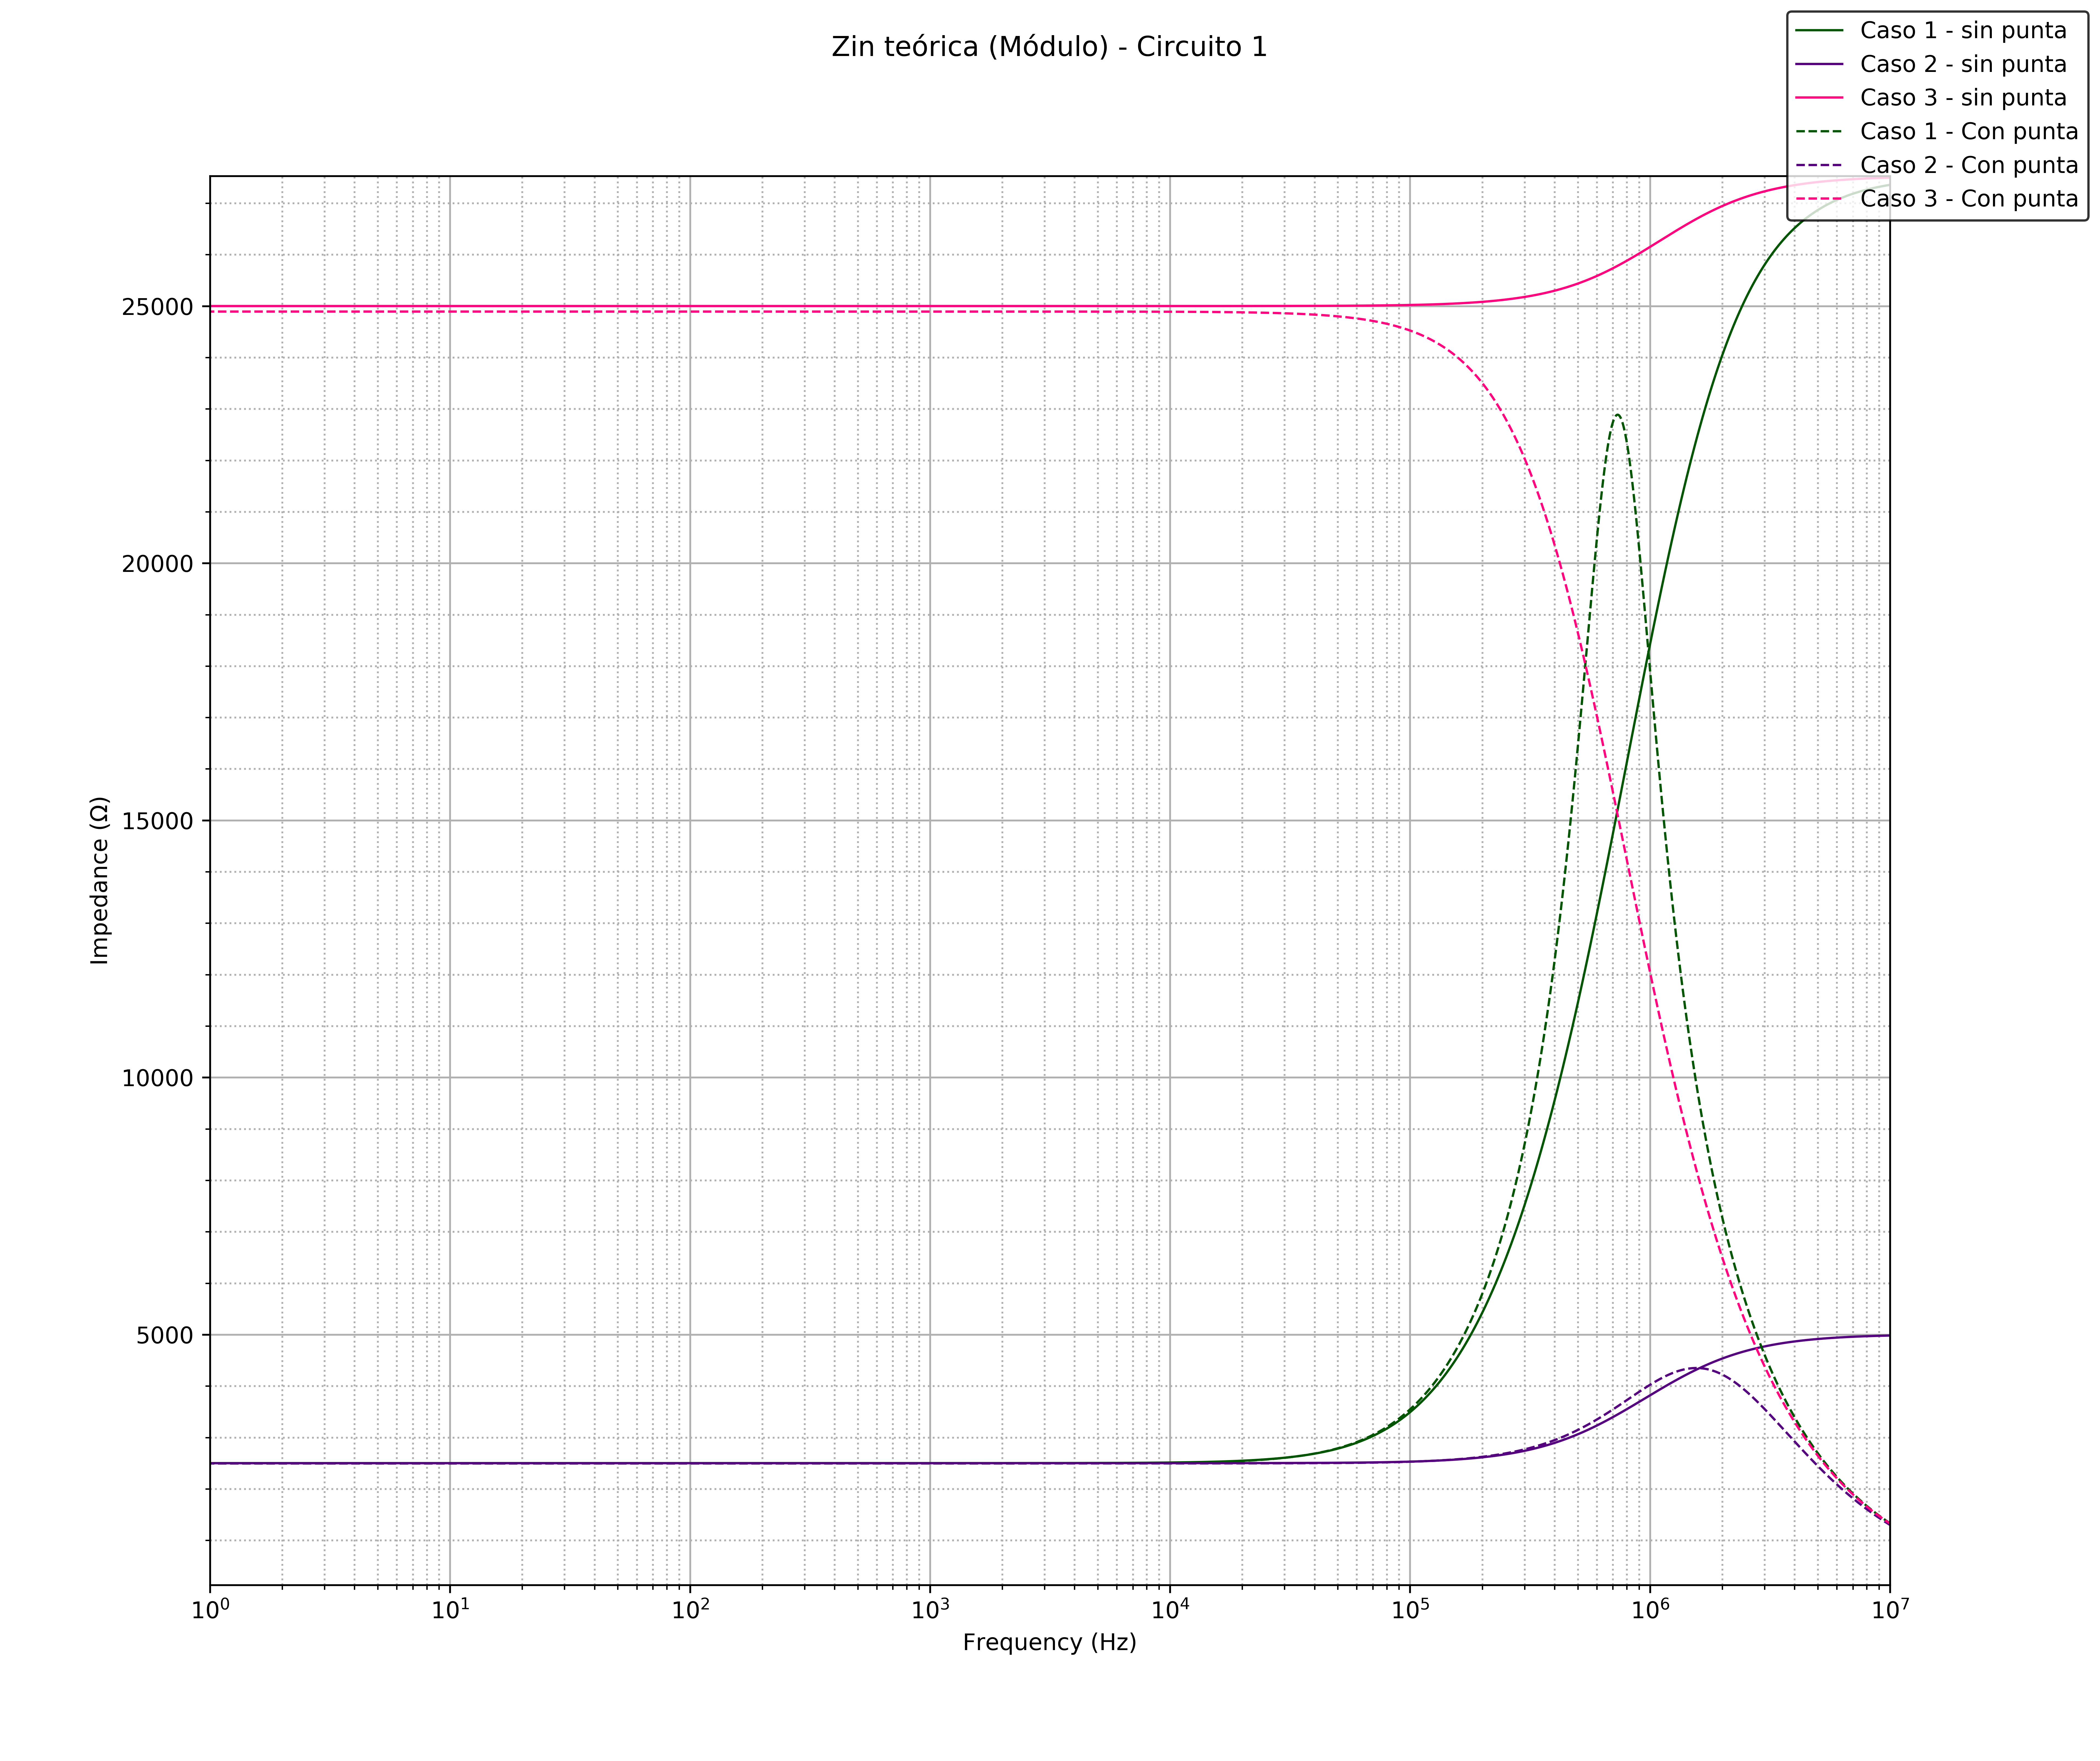
\includegraphics[width=10cm,height=10cm,keepaspectratio]{../EJ1/00GRAFICOS/teoricos/c1zinm.png}
	\caption{Configuración inversora - M\'odulo de $Z_{in}$ calculada de forma te\'orica con y sin punta del osciloscopio.}
	\label{c1zintm}
\end{figure}

\begin{figure}[H] %!ht
	\centering
	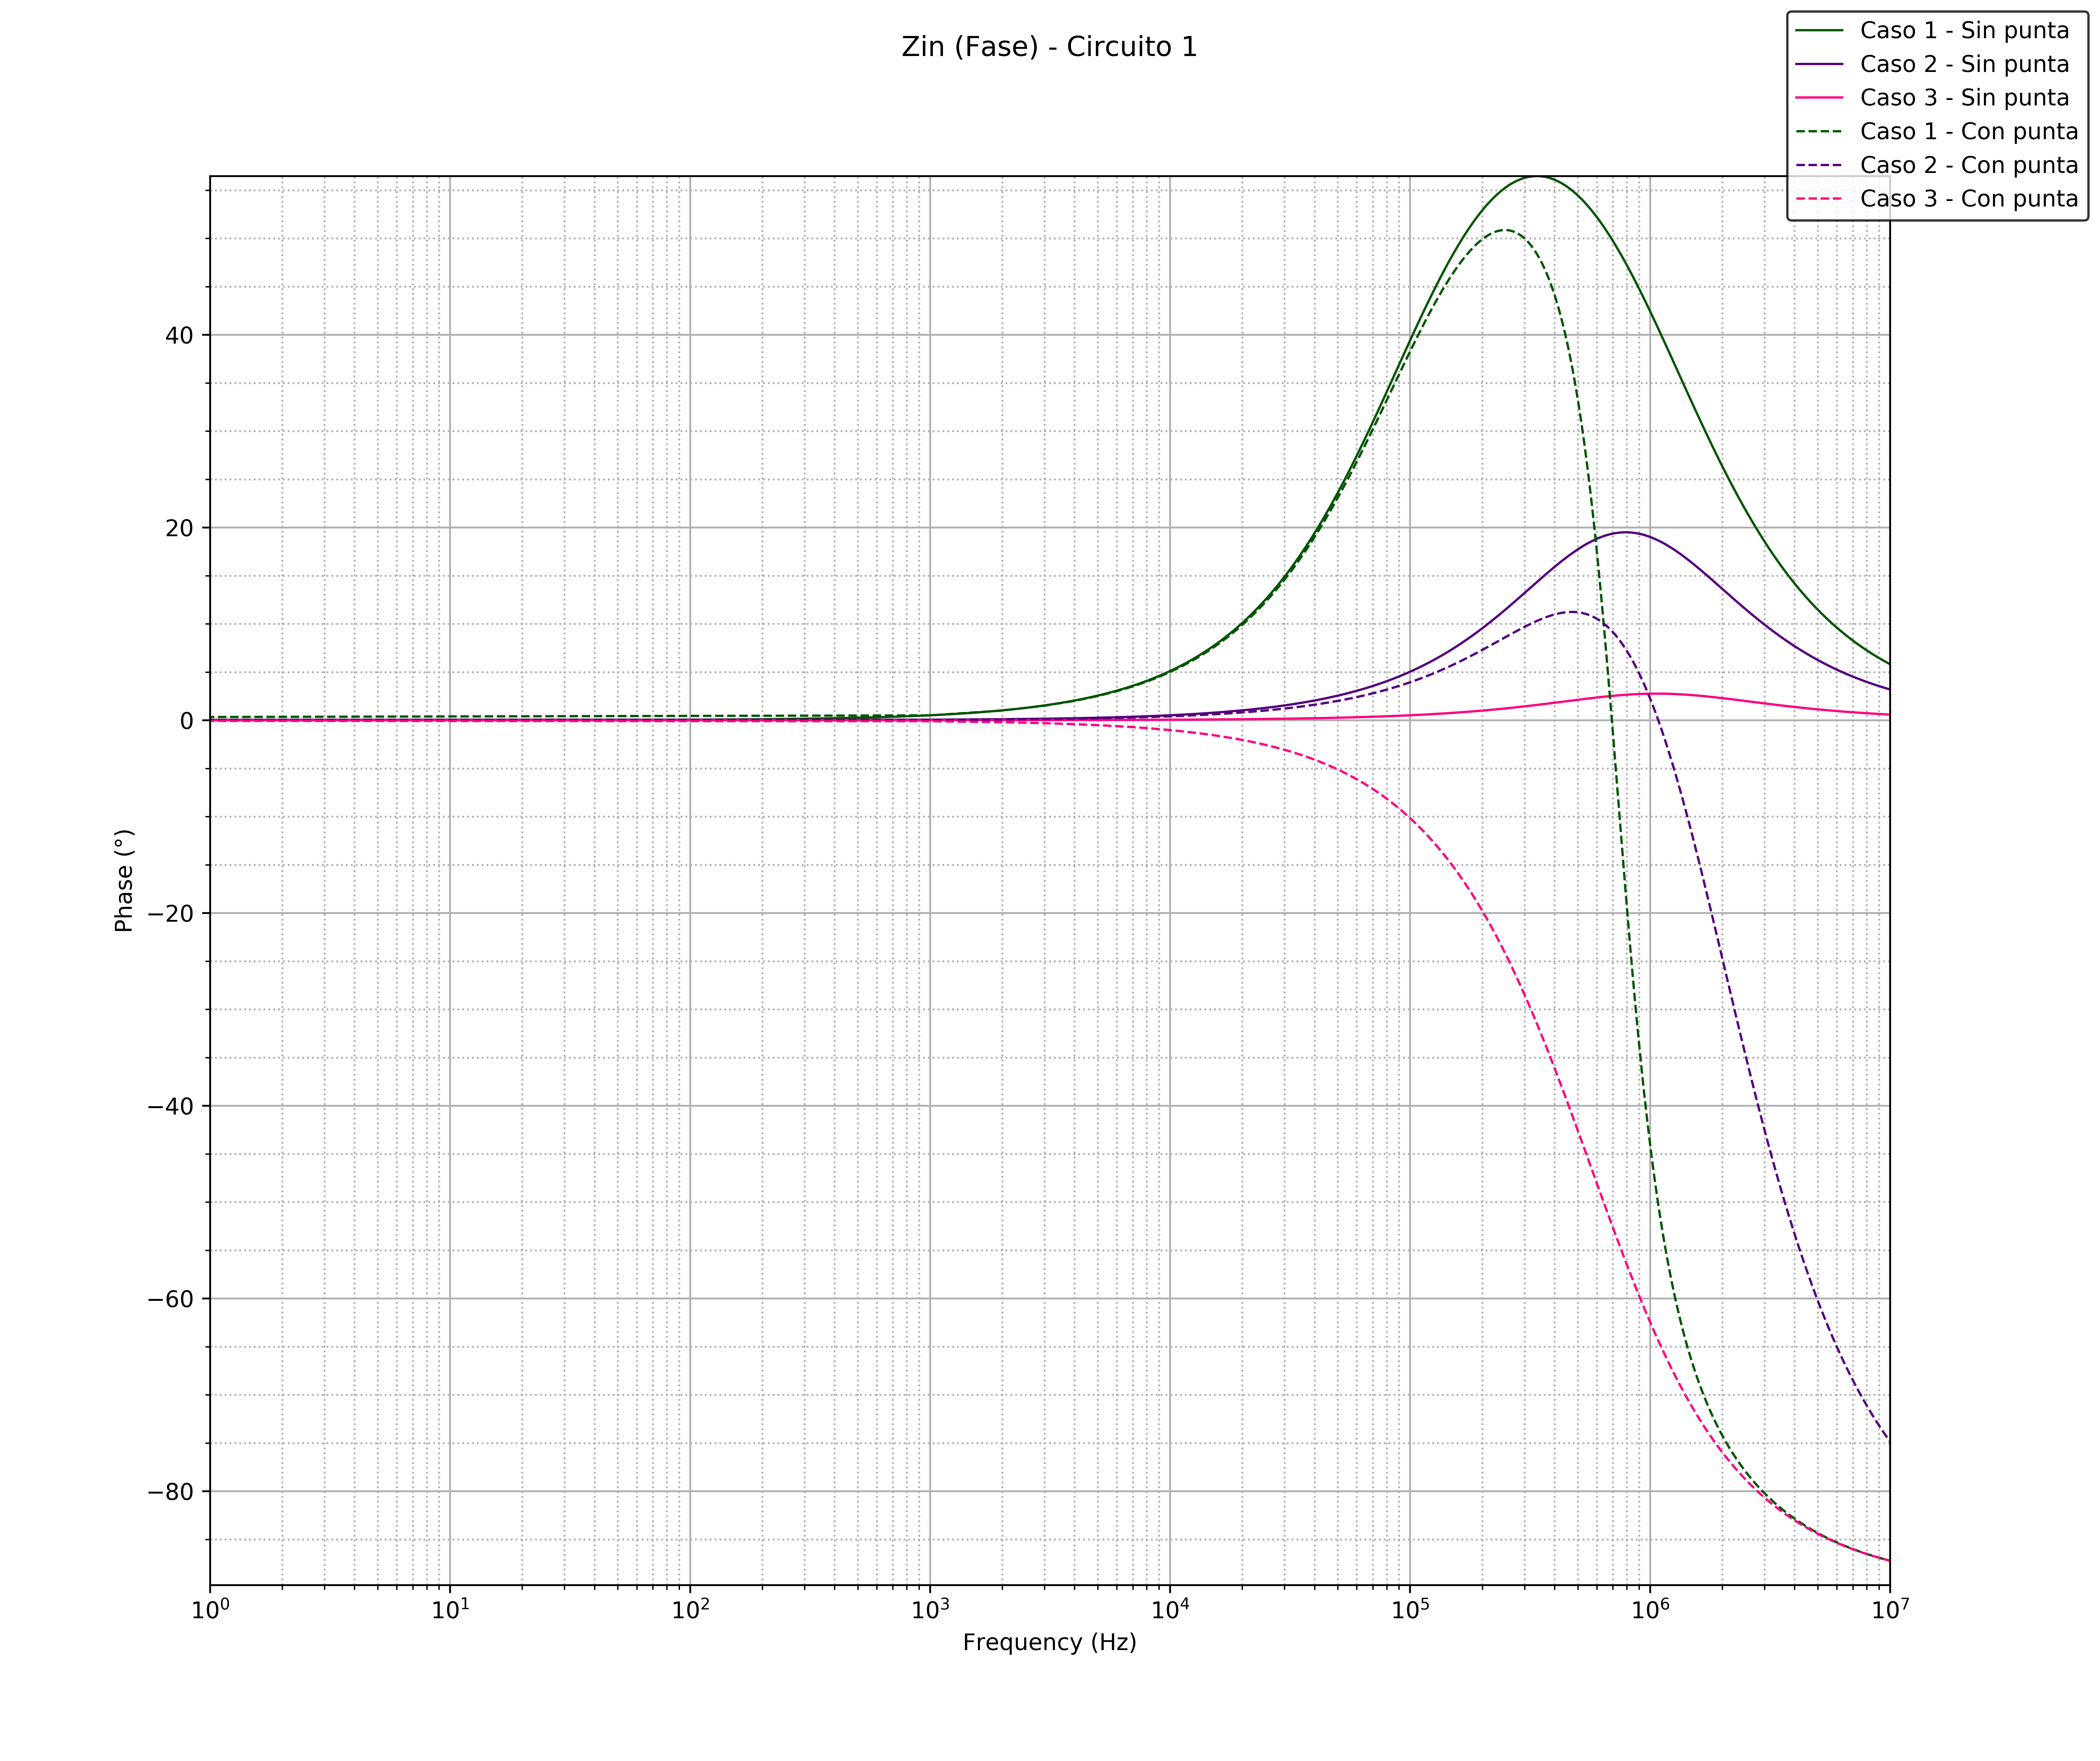
\includegraphics[width=10cm,height=10cm,keepaspectratio]{../EJ1/00GRAFICOS/teoricos/circ1zinfases.png}
	\caption{Configuración inversora - Fase de $Z_{in}$ calculada de forma te\'orica con y sin la punta del osciloscopio.}
	\label{c1zintp}
\end{figure}
%hablar de las diferencias entre cada caso

\subsubsection*{Configuraci\'on no inversora}

Los c\'alculos te\'oricos que se llevaron a cabo para la impedancia de entrada del circuitode configuraci\'on no inversora \ref{c2} son an\'alogos a los realizados para el circuito inversor \ref{c1}. La expresi\'on \ref{c2zint} corresponde a c\'alculo te\'orico que se hizo sin tener en cuenta la punta del osciloscopio:

\begin{equation}
	Z_{in} =  R_3 + R_4
	\label{c2zint}
\end{equation}

Reemplazando con los valores de resistencias correspondientes a cada caso (Ver tabla \ref{casos}), se obtienen las siguientes impedancia de entrada:

Casos 1 y 2:
\begin{equation}
	Z_{in} =  12,5k\Omega
	\label{c2c1zint}
\end{equation}

caso 3:
\begin{equation}
	Z_{in} =  125k\Omega
	\label{c3c3zint}
\end{equation}

Como el circuito es resistivo y la expresi\'on \ref{c2zint} no depende de $A_{vol}$, la impedancia de entrada se mantiene constante para todas las frecuencias. Sin embargo, a continuaci\'on se muestra la expresi\'on obtenida al hacer el c\'alculo considerando la punta del osciloscopio a la entrada, lo cual permite ver que de esa forma deja de mantenerse constante la impedancia previamente calculada.


\begin{equation}
	Z_{in}\rvert_{c/punta} = 8,33 \cdot 10^{17} \cdot (R3 + R4)/((R3 + R4) \cdot (10^7 s + 8,33 \cdot 10^{10}) + 8,33 \cdot 10^{17})
	\label{zinp}
\end{equation}

Si bien la expresi\'on del c\'alculo con la punta del osciloscopio, \ref{zinp}, sigue sin depender de $A_{vol}$, var\'ia con la frecuencia ya que el modelo de la punta tiene un capacitor.

Evaluando para cada uno de los casos indicados en la tabla \ref{casos}, se llega a las siguientes expresiones para la impedancia de entrada incluyendo la punta X10 del osciloscopio $Z_{in}\rvert_{c/punta}$:

Casos 1 y 2:
\begin{equation}
	Z_{in}\rvert_{c/punta} = \frac{1,04 \cdot 10^22}{1,25 \cdot 10^11 + 8.34 \cdot 10^17}
	\label{c2c1zinp}
\end{equation}

Caso 3:
\begin{equation}
	Z_{in}\rvert_{c/punta} = \frac{1,04 \cdot 10^23}{1,25 \cdot 10^12 + 8,43 \cdot 10^17}
	\label{c2c3zinp}
\end{equation}


A continuaci\'on, en los gr\'aficos \ref{c2zintm} y \ref{c2zintp} se muestra la impedancia de entrada del circuito calculada de forma te\'orica con y sin punta del osciloscopio para los tres casos de la tabla \ref{casos}:

\begin{figure}[H] %!ht
	\centering
	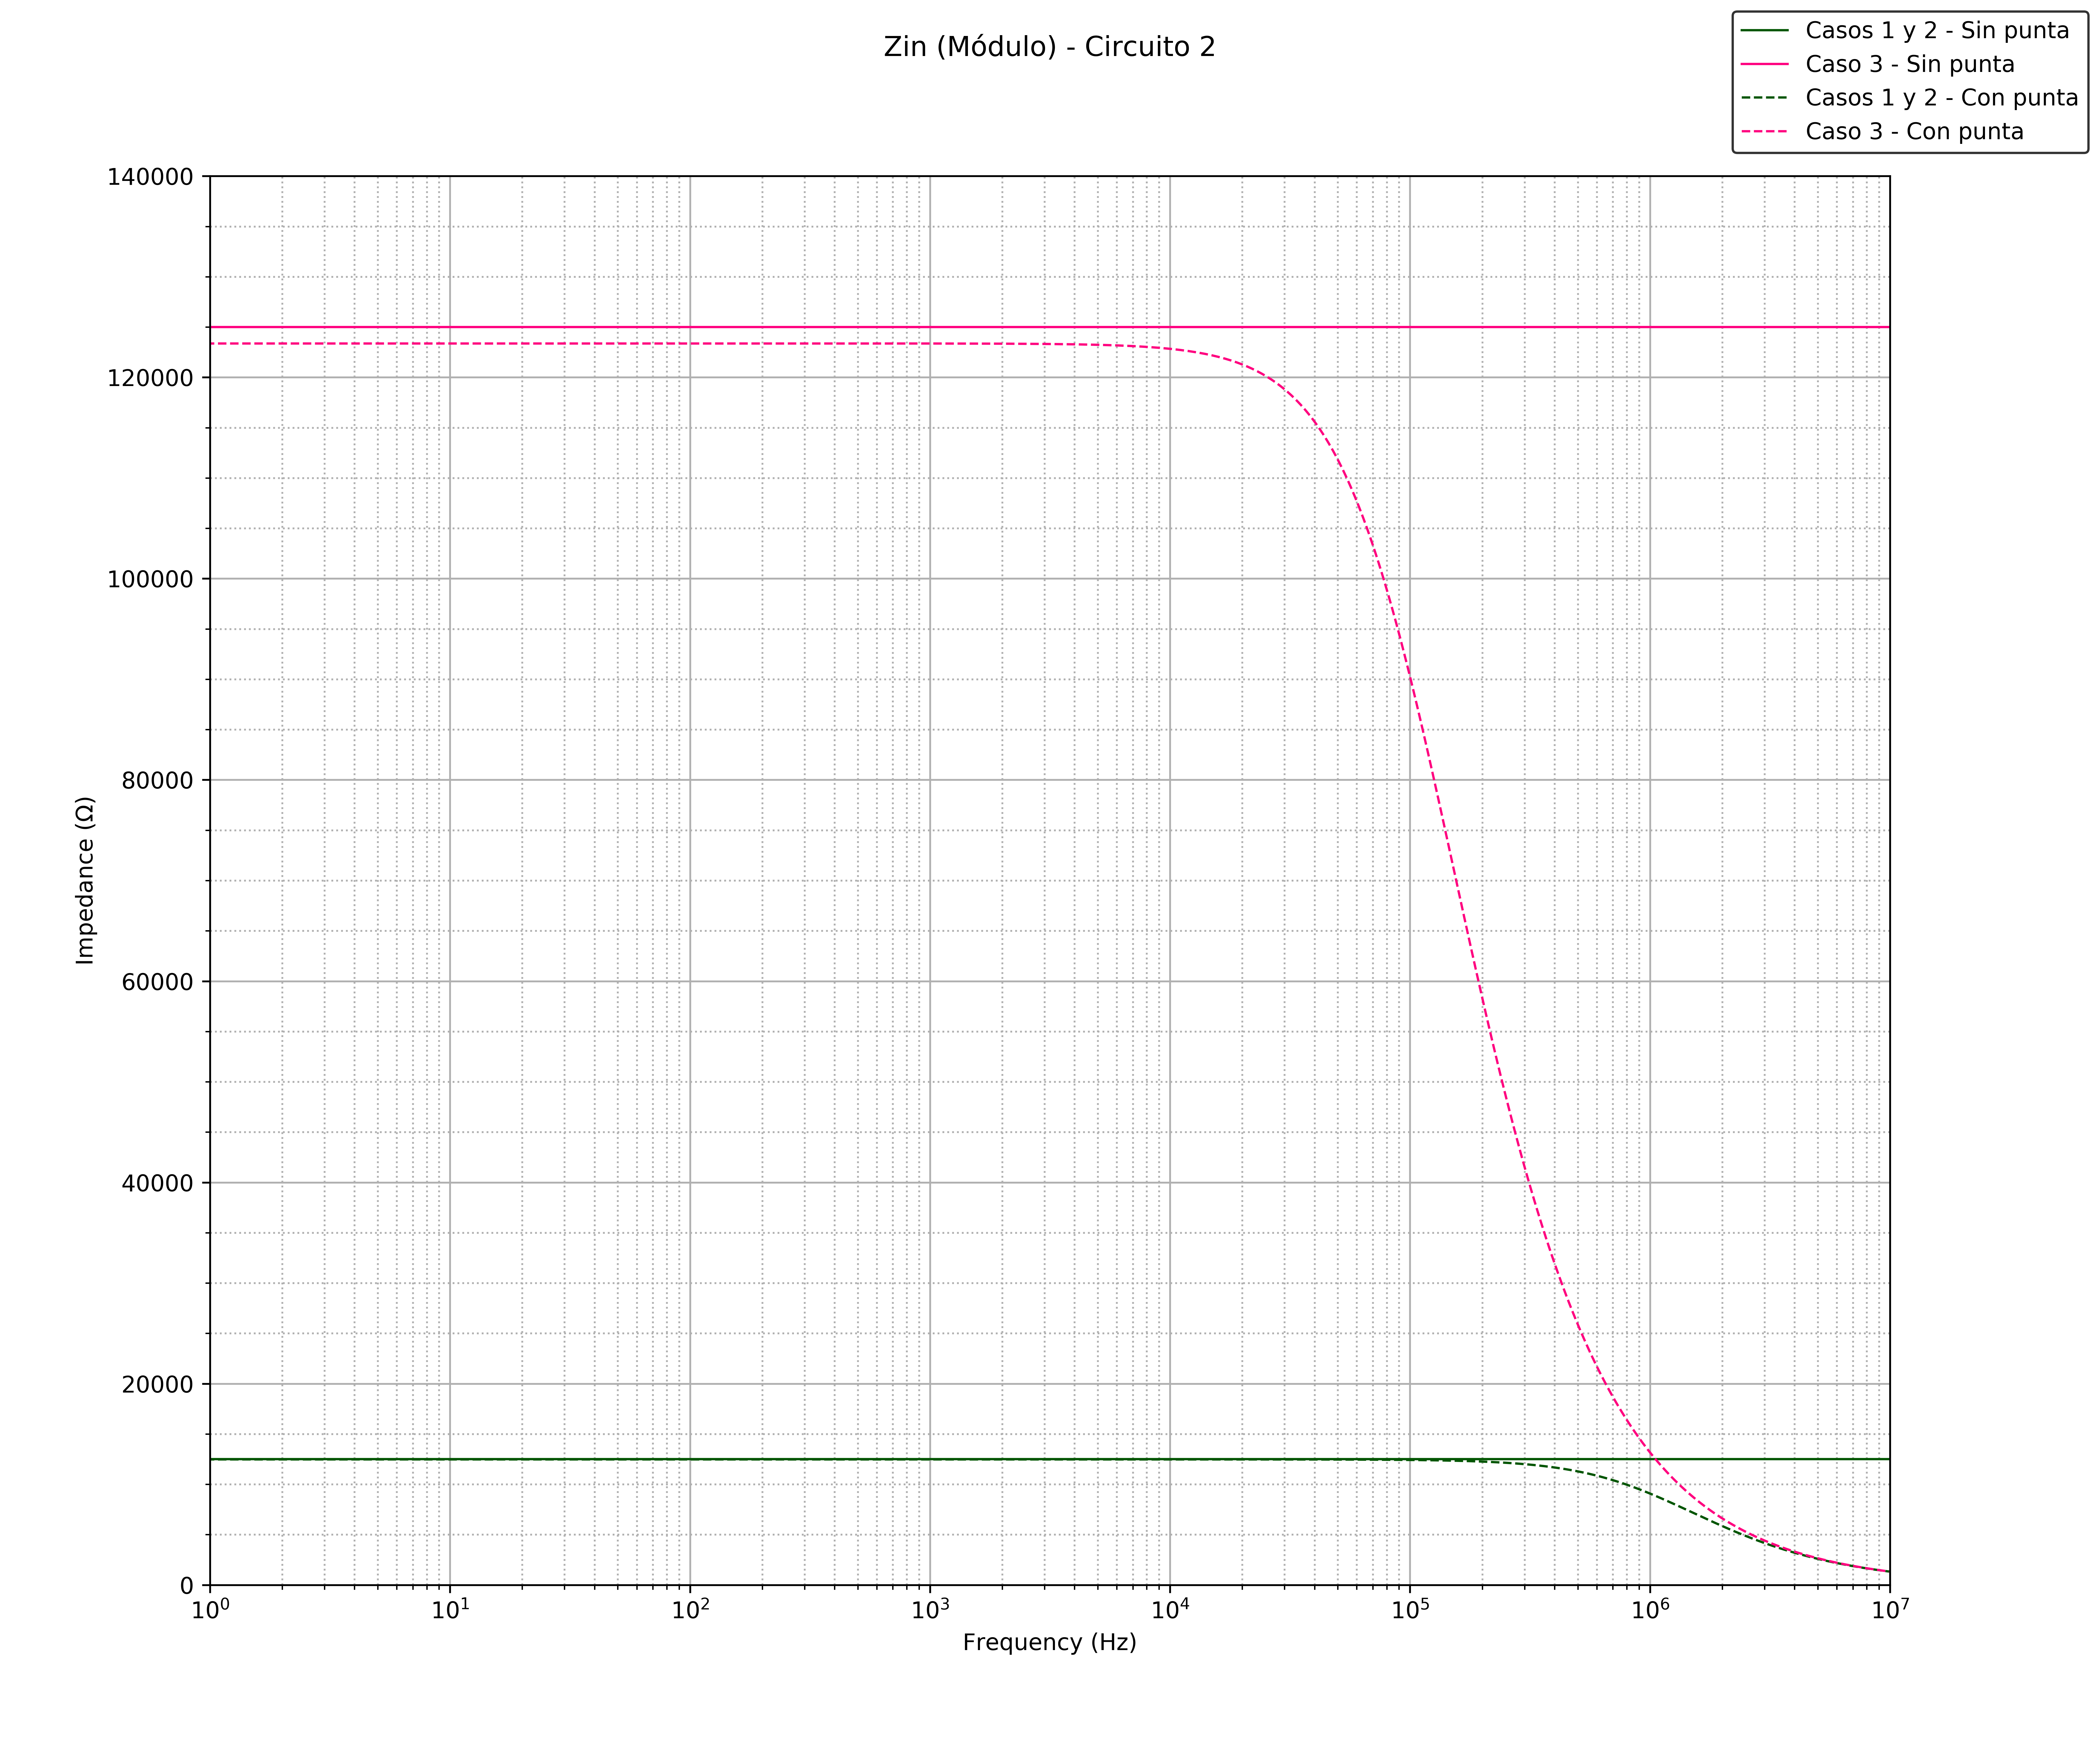
\includegraphics[width=10cm,height=10cm,keepaspectratio]{../EJ1/00GRAFICOS/teoricos/circ2zinm.png}
	\caption{Configuración inversora - M\'odulo de $Z_{in}$ calculada de forma te\'orica con y sin punta del osciloscopio.}
	\label{c2zintm}
\end{figure}

\begin{figure}[H] %!ht
	\centering
	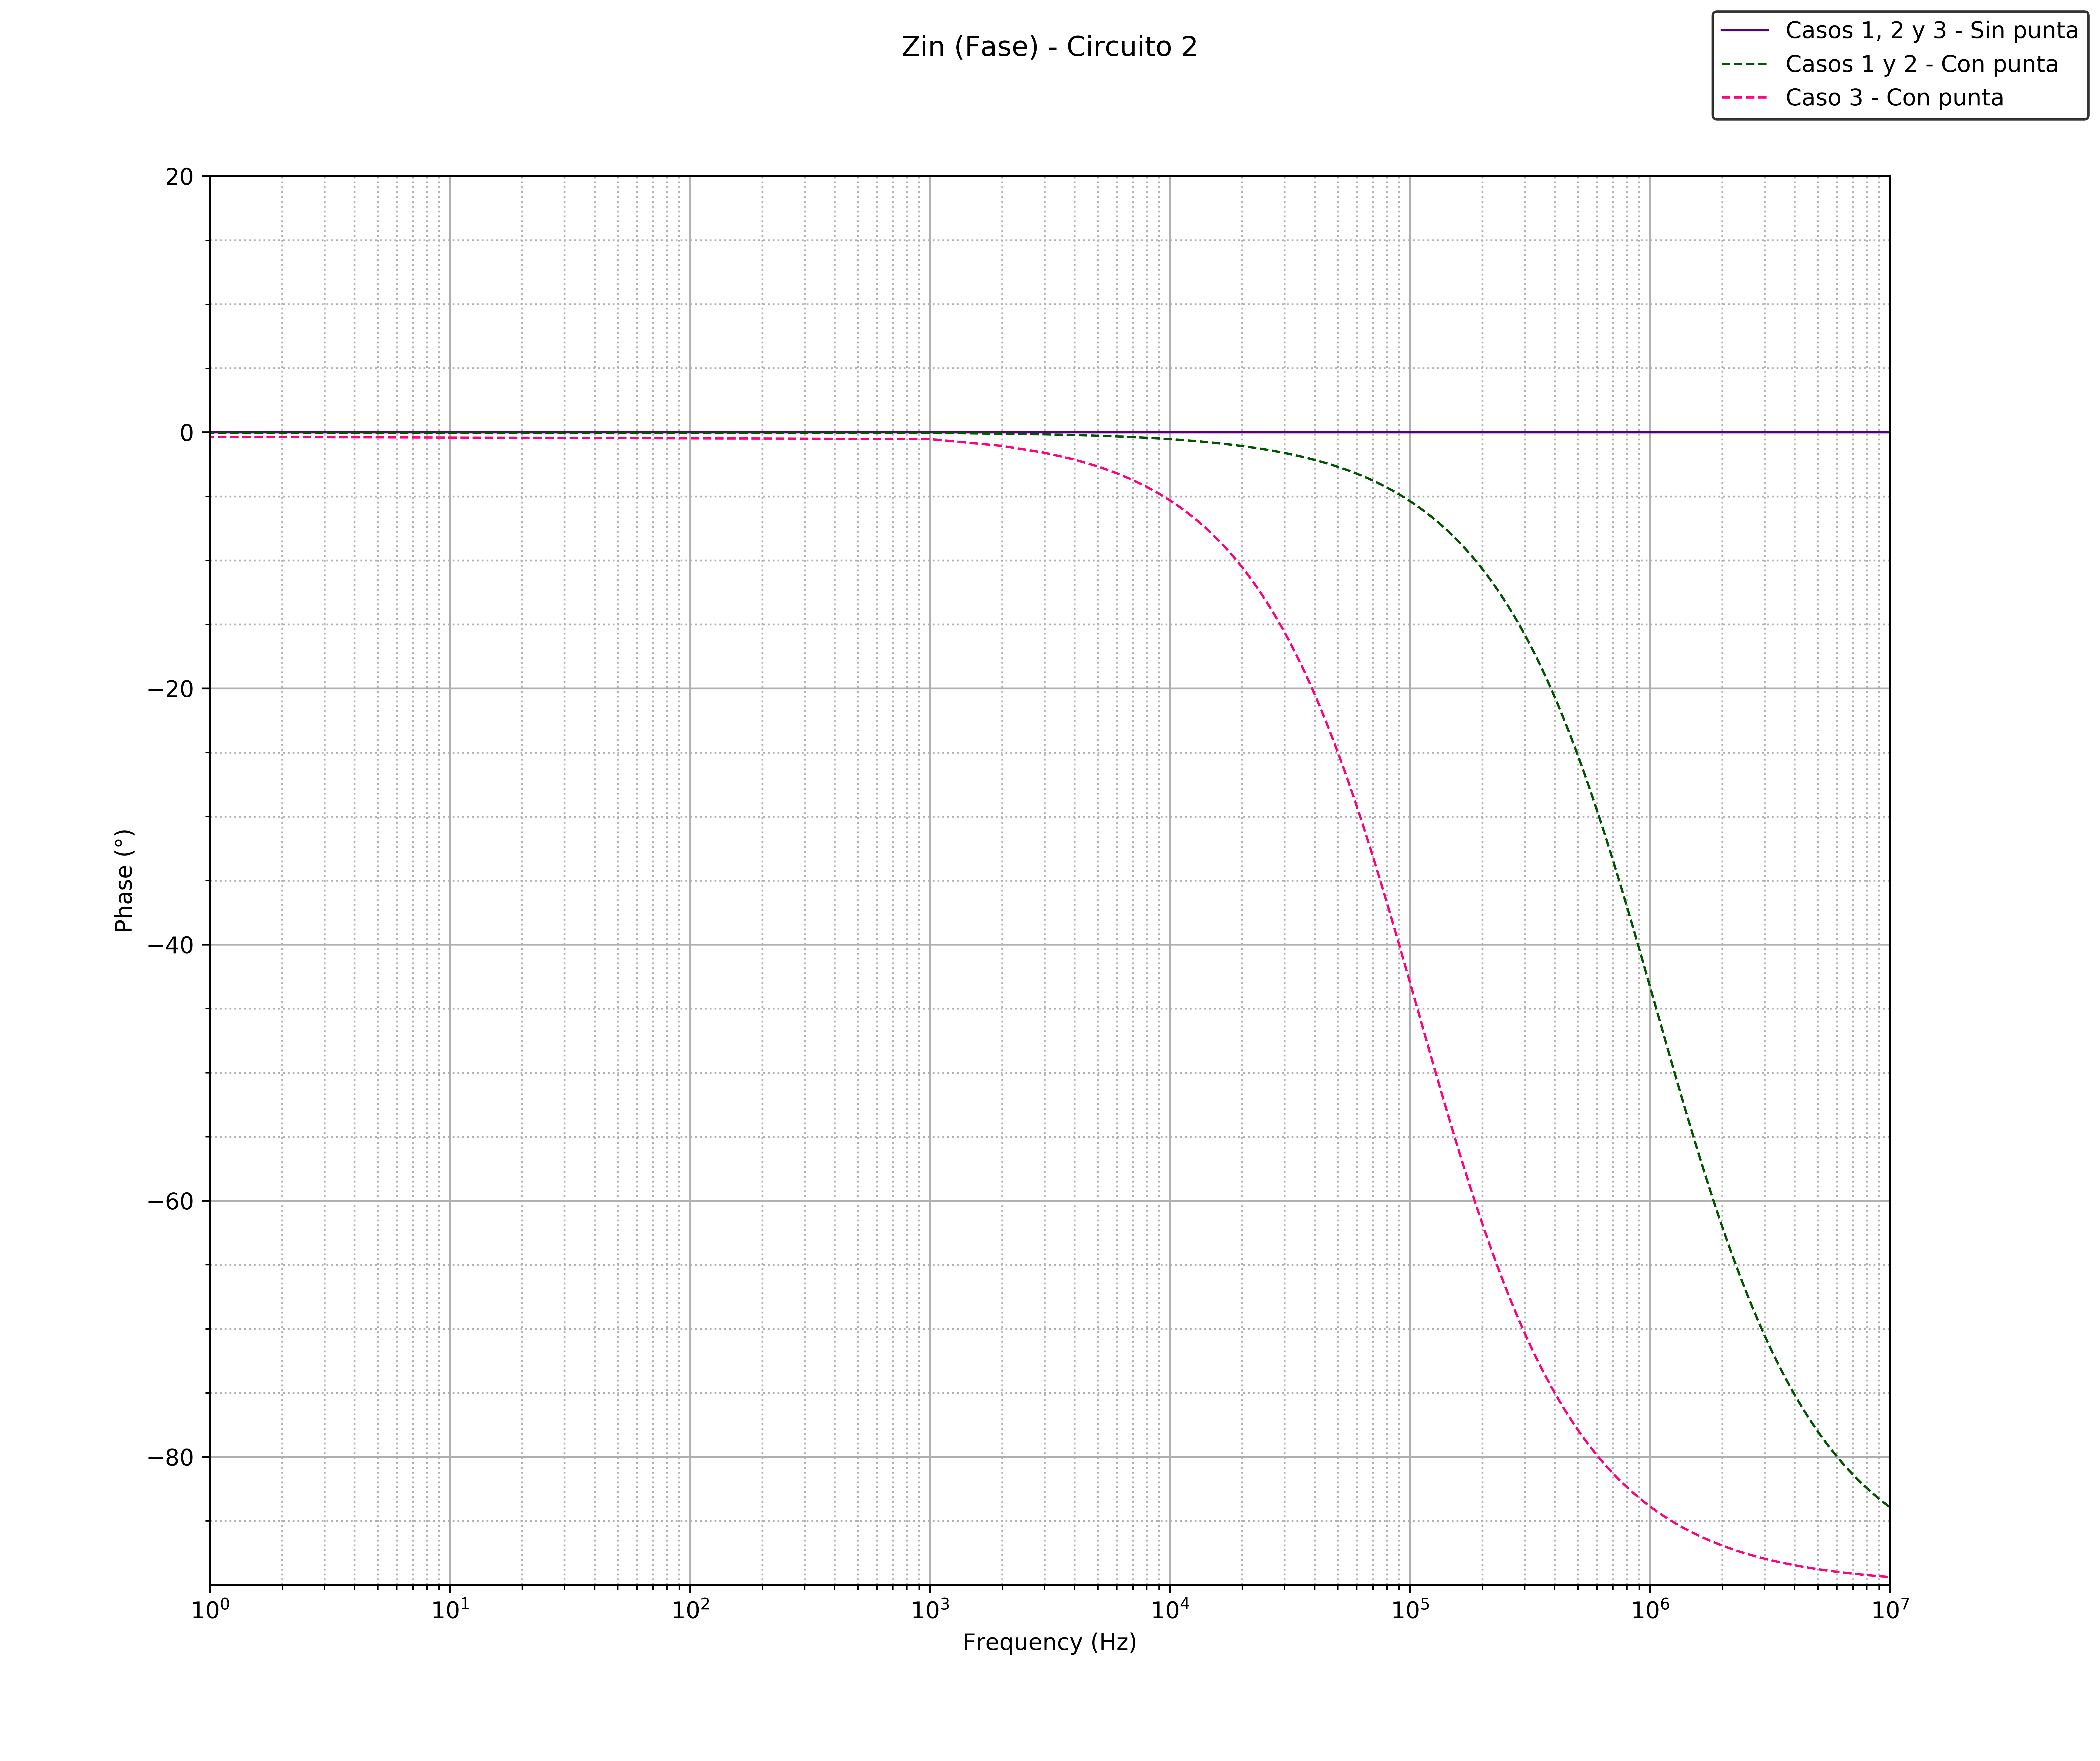
\includegraphics[width=10cm,height=10cm,keepaspectratio]{../EJ1/00GRAFICOS/teoricos/circ2zinfase.png}
	\caption{Configuración inversora - Fase de $Z_{in}$ calculada de forma te\'orica con y sin la punta del osciloscopio.}
	\label{c2zintp}
\end{figure}
%hablar de las diferencias entre cada caso

\subsubsection{Mediciones y resultados obtenidos} %%%%%%



\subsubsection*{Configuraci\'on inversora}
Para medir la impedancia de entrada del circuito en funci\'on de la frecuencia, 
deb\'iamos hacer el cociente $V_{in}/I_{in}$. Si bien se puede medir la tensi\'on 
de entrada al circuito de forma directa con el osciloscopio, 
no es tan sensillo obtener la corriente que entra al circuito, ya que el osciloscopio 
mide tensiones y no corrientes. Se busc\'o una resistencia $R_L$ cuyo valor comerical 
fuera lo m\'as parecido posible (igual o el primero mayor) al valor obtenido en 
el c\'alculo te\'rico para cada uno de los casos de resistencias. Se coloc\'o dicha 
resistencia en serie al generador, a la entrada del circuito. Luego se midi\'o la ca\'ida 
de tensi\'on sobre ella, ya que al dividirla por el valor de la $R_L$ colocada se obtendr\'ia 
la corriente de entrada al circuito $I_{in}$. El criterio de buscar una resistencia similar 
al valor calculado de $Z_{in}$ surge de que si se pusiese una resistencia muy chica, 
la diferencia entre las tensiones medidas sobre sus bornes ser\'ia muy chica 
(aumentando incertidumbre) y si se colocase una resistencia muy grande, 
la tensi\'on que caer\'ia ser\'ia mucho mayor a la que caer\'ia en el circuito, 
haciendo que la tensi\'on luego de la resistencia sea muy chica (se podr\'ia 
acercar al nivel de ruido) y que la diferencia de tensi\'on entre sus bornes tienda 
a la tensi\'on entregada por el generador. Por eso se consider\'o \'optimo que la 
resistencia tenga un valor similar al calculado de forma te\'orica y en caso de no 
conseguir el mismo valor, prefiri\'endose un valor mayor y no menor. 

\begin{figure}[H] %!ht
	\centering
	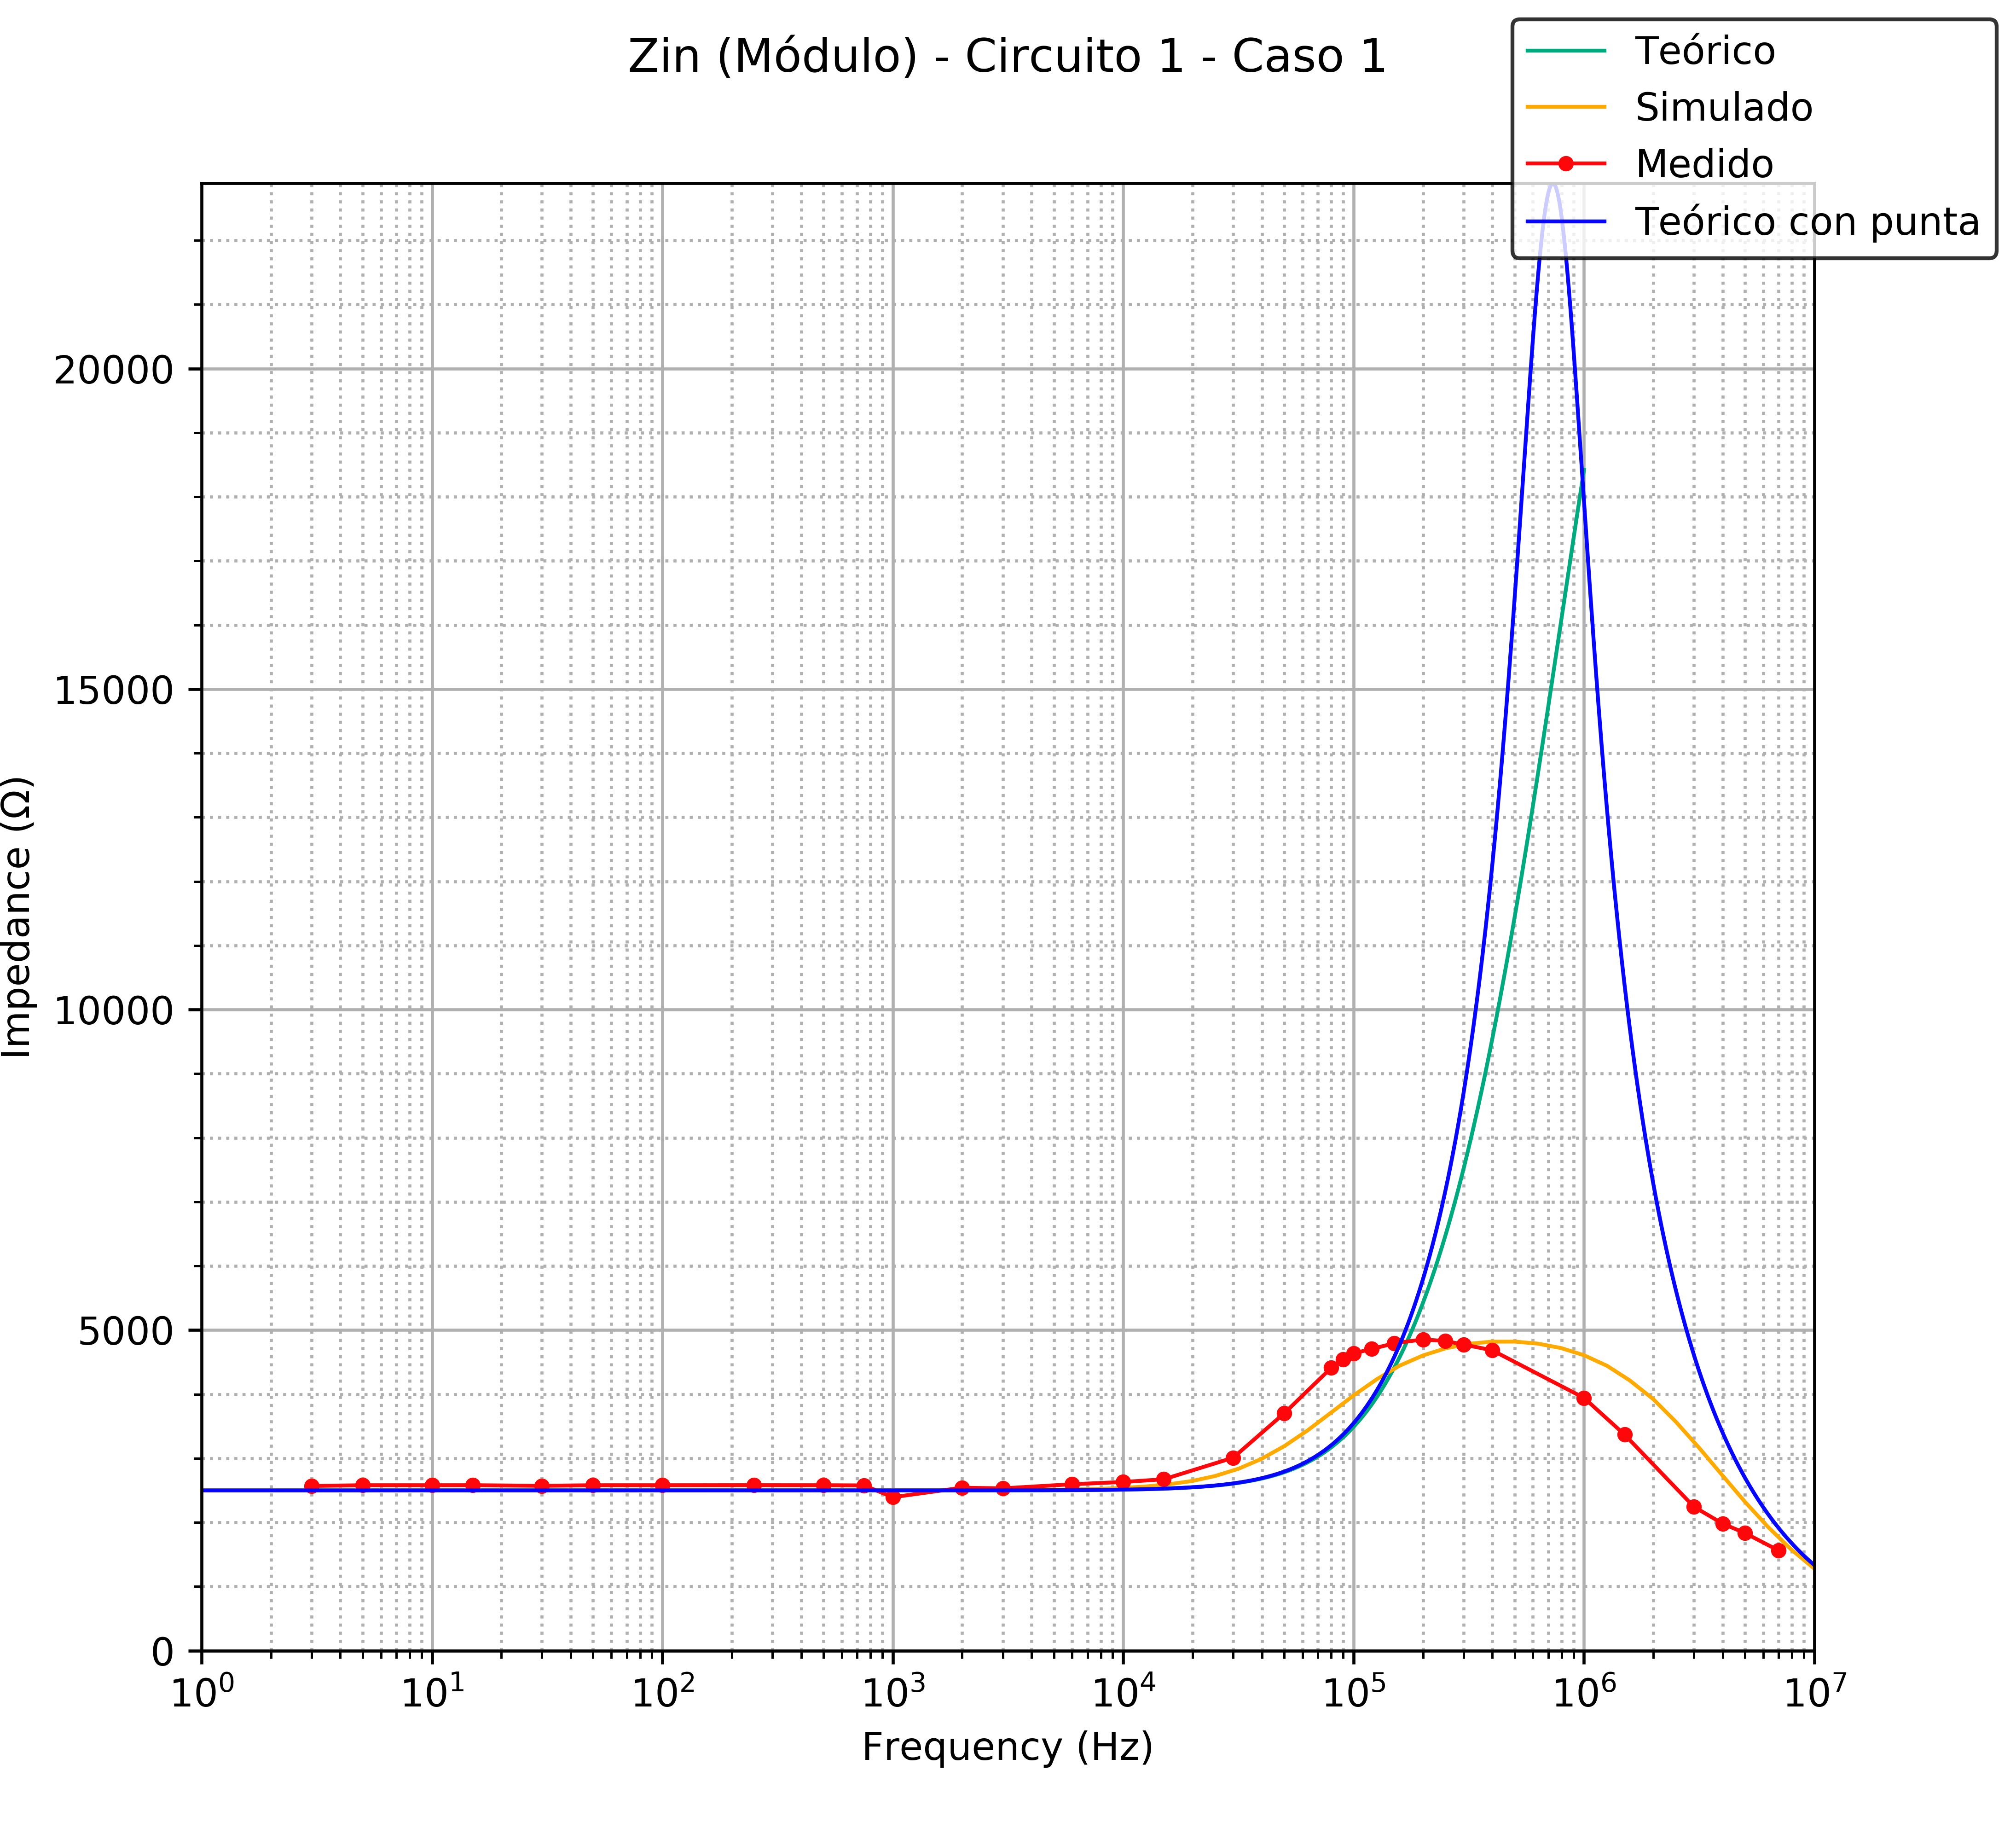
\includegraphics[width=10cm,height=10cm,keepaspectratio]{../EJ1/00GRAFICOS/c1c1/c1c1ZINpunta.png}
	\caption{Configuración inversora - Caso 1 - M\'odulo de $Z_{in}$}
	\label{c1c1zinM}
\end{figure}

\begin{figure}[H] %!ht
	\centering
	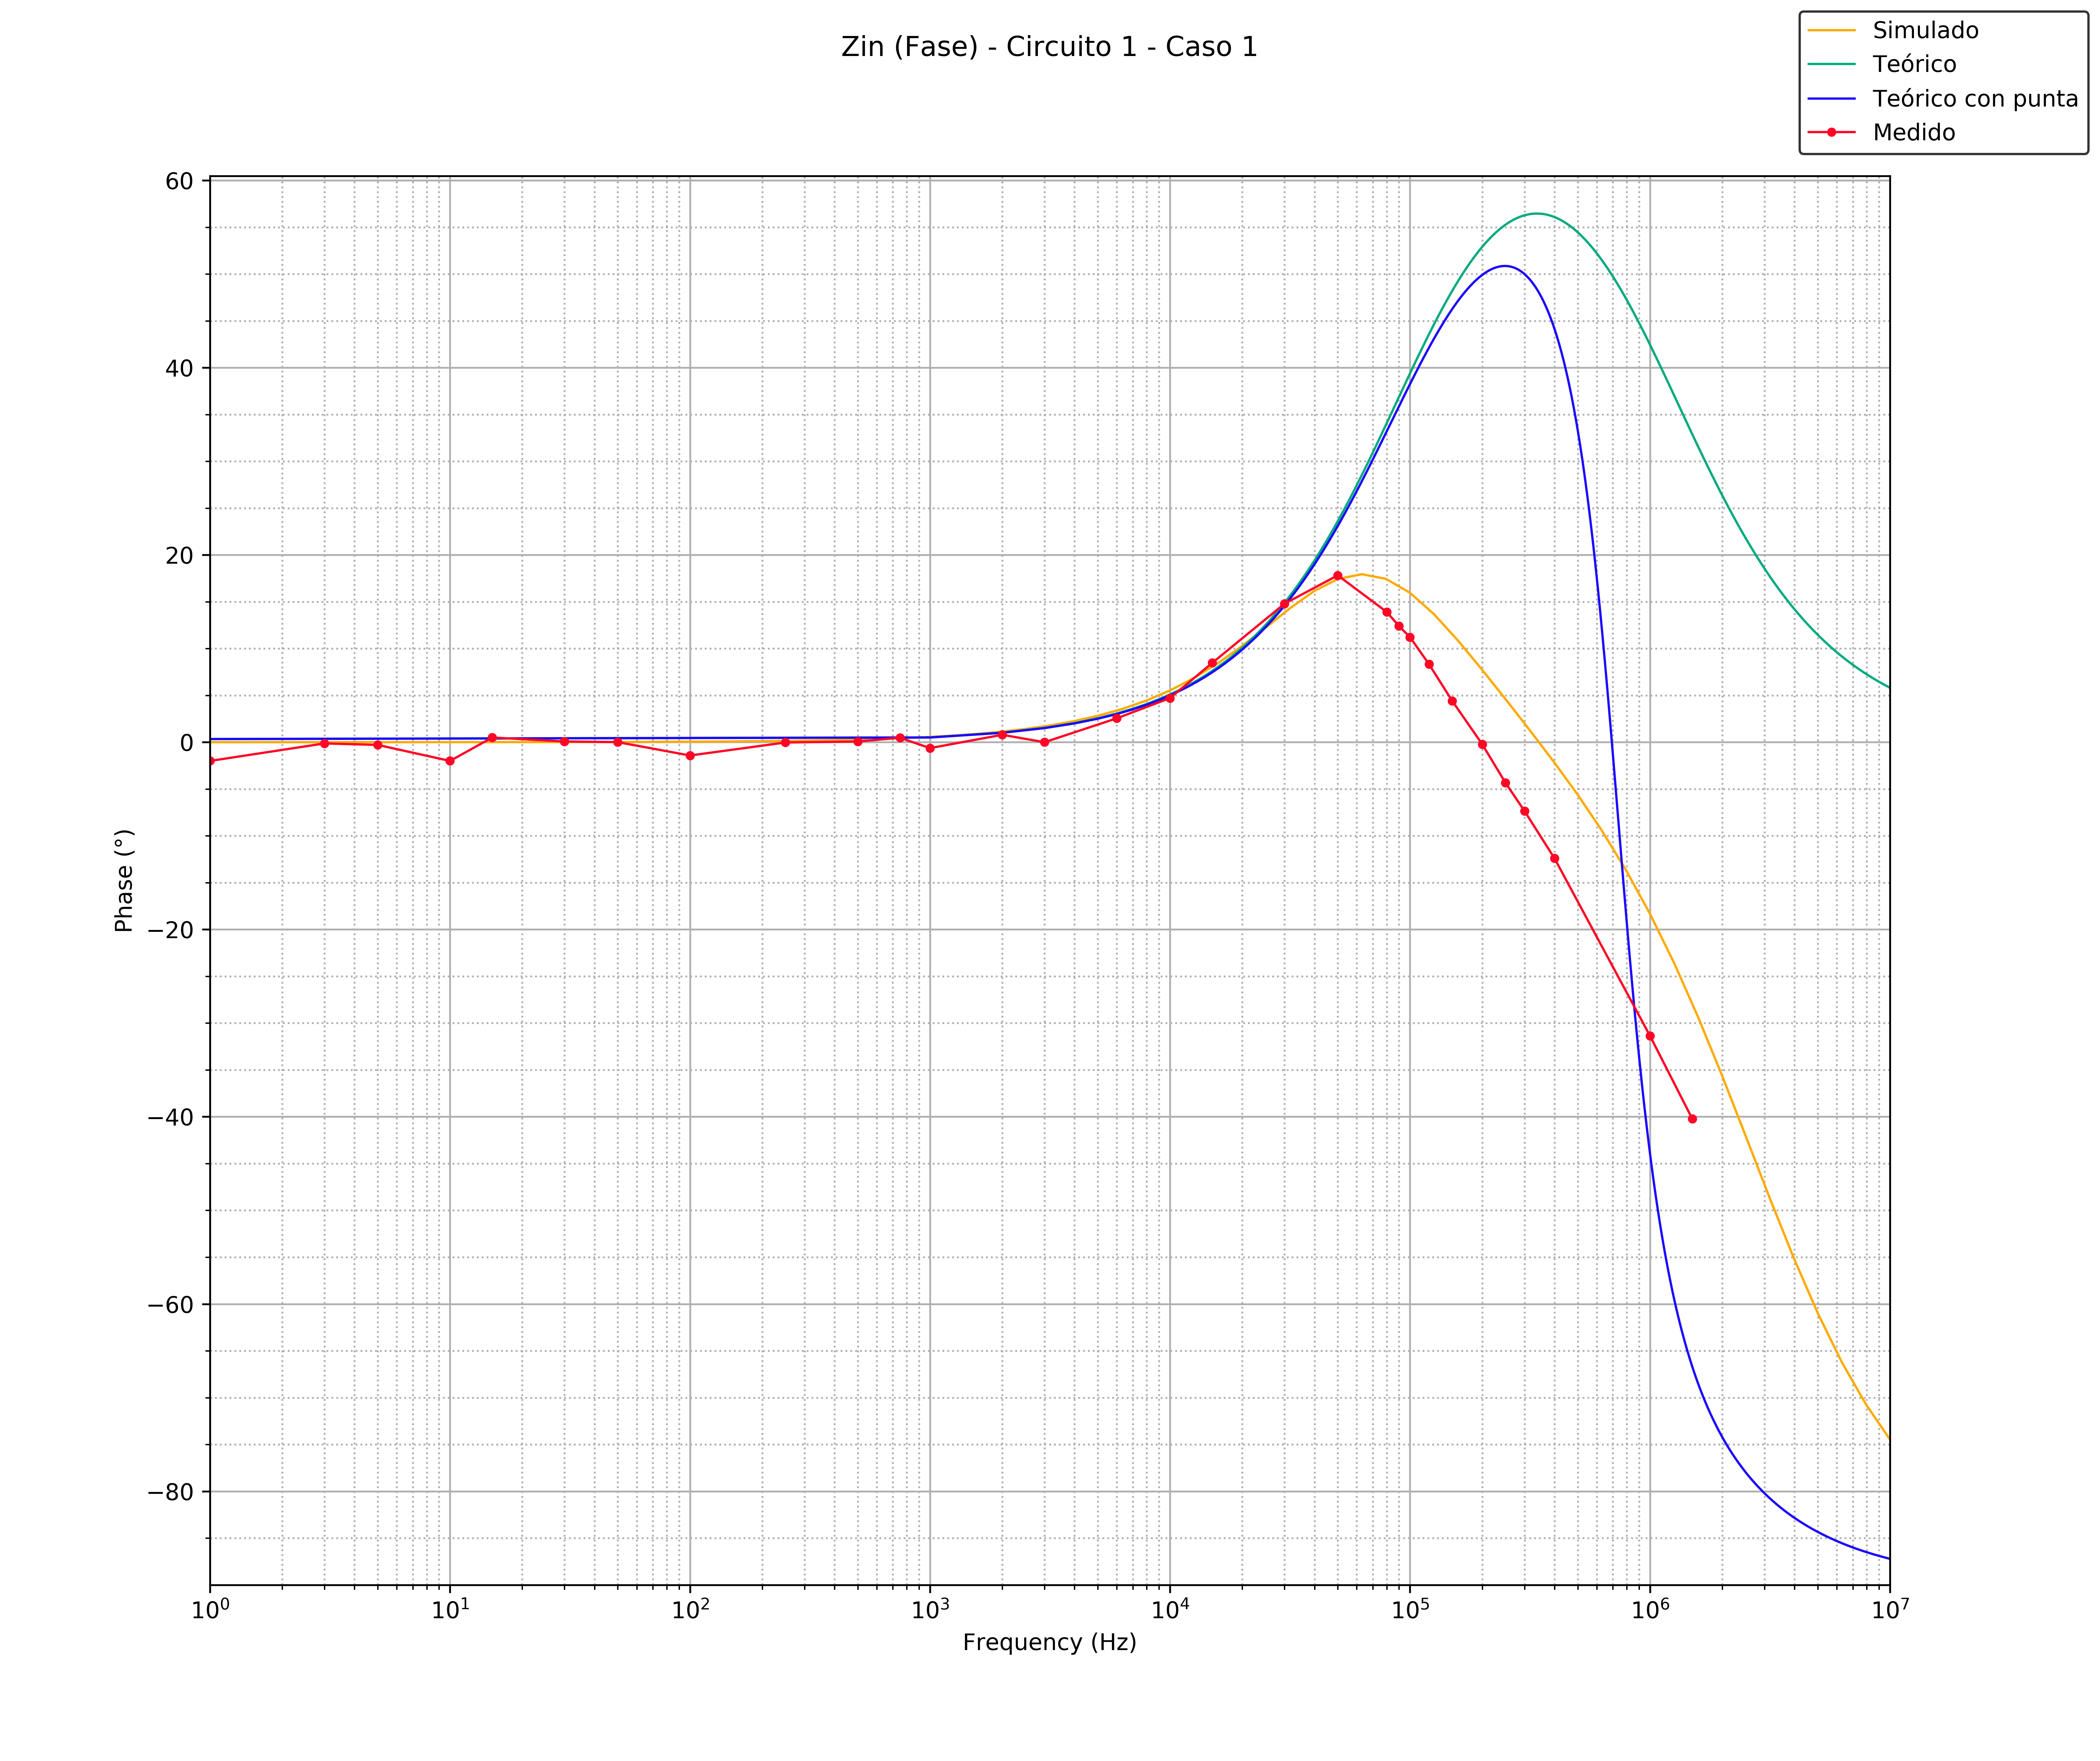
\includegraphics[width=10cm,height=10cm,keepaspectratio]{../EJ1/00GRAFICOS/c1c1/c1c1zinFASE.png}
	\caption{Configuración inversora - Caso 1 - Fase de $Z_{in}$ }
	\label{c1c1zinP}
\end{figure}

\begin{figure}[H] %!ht
	\centering
	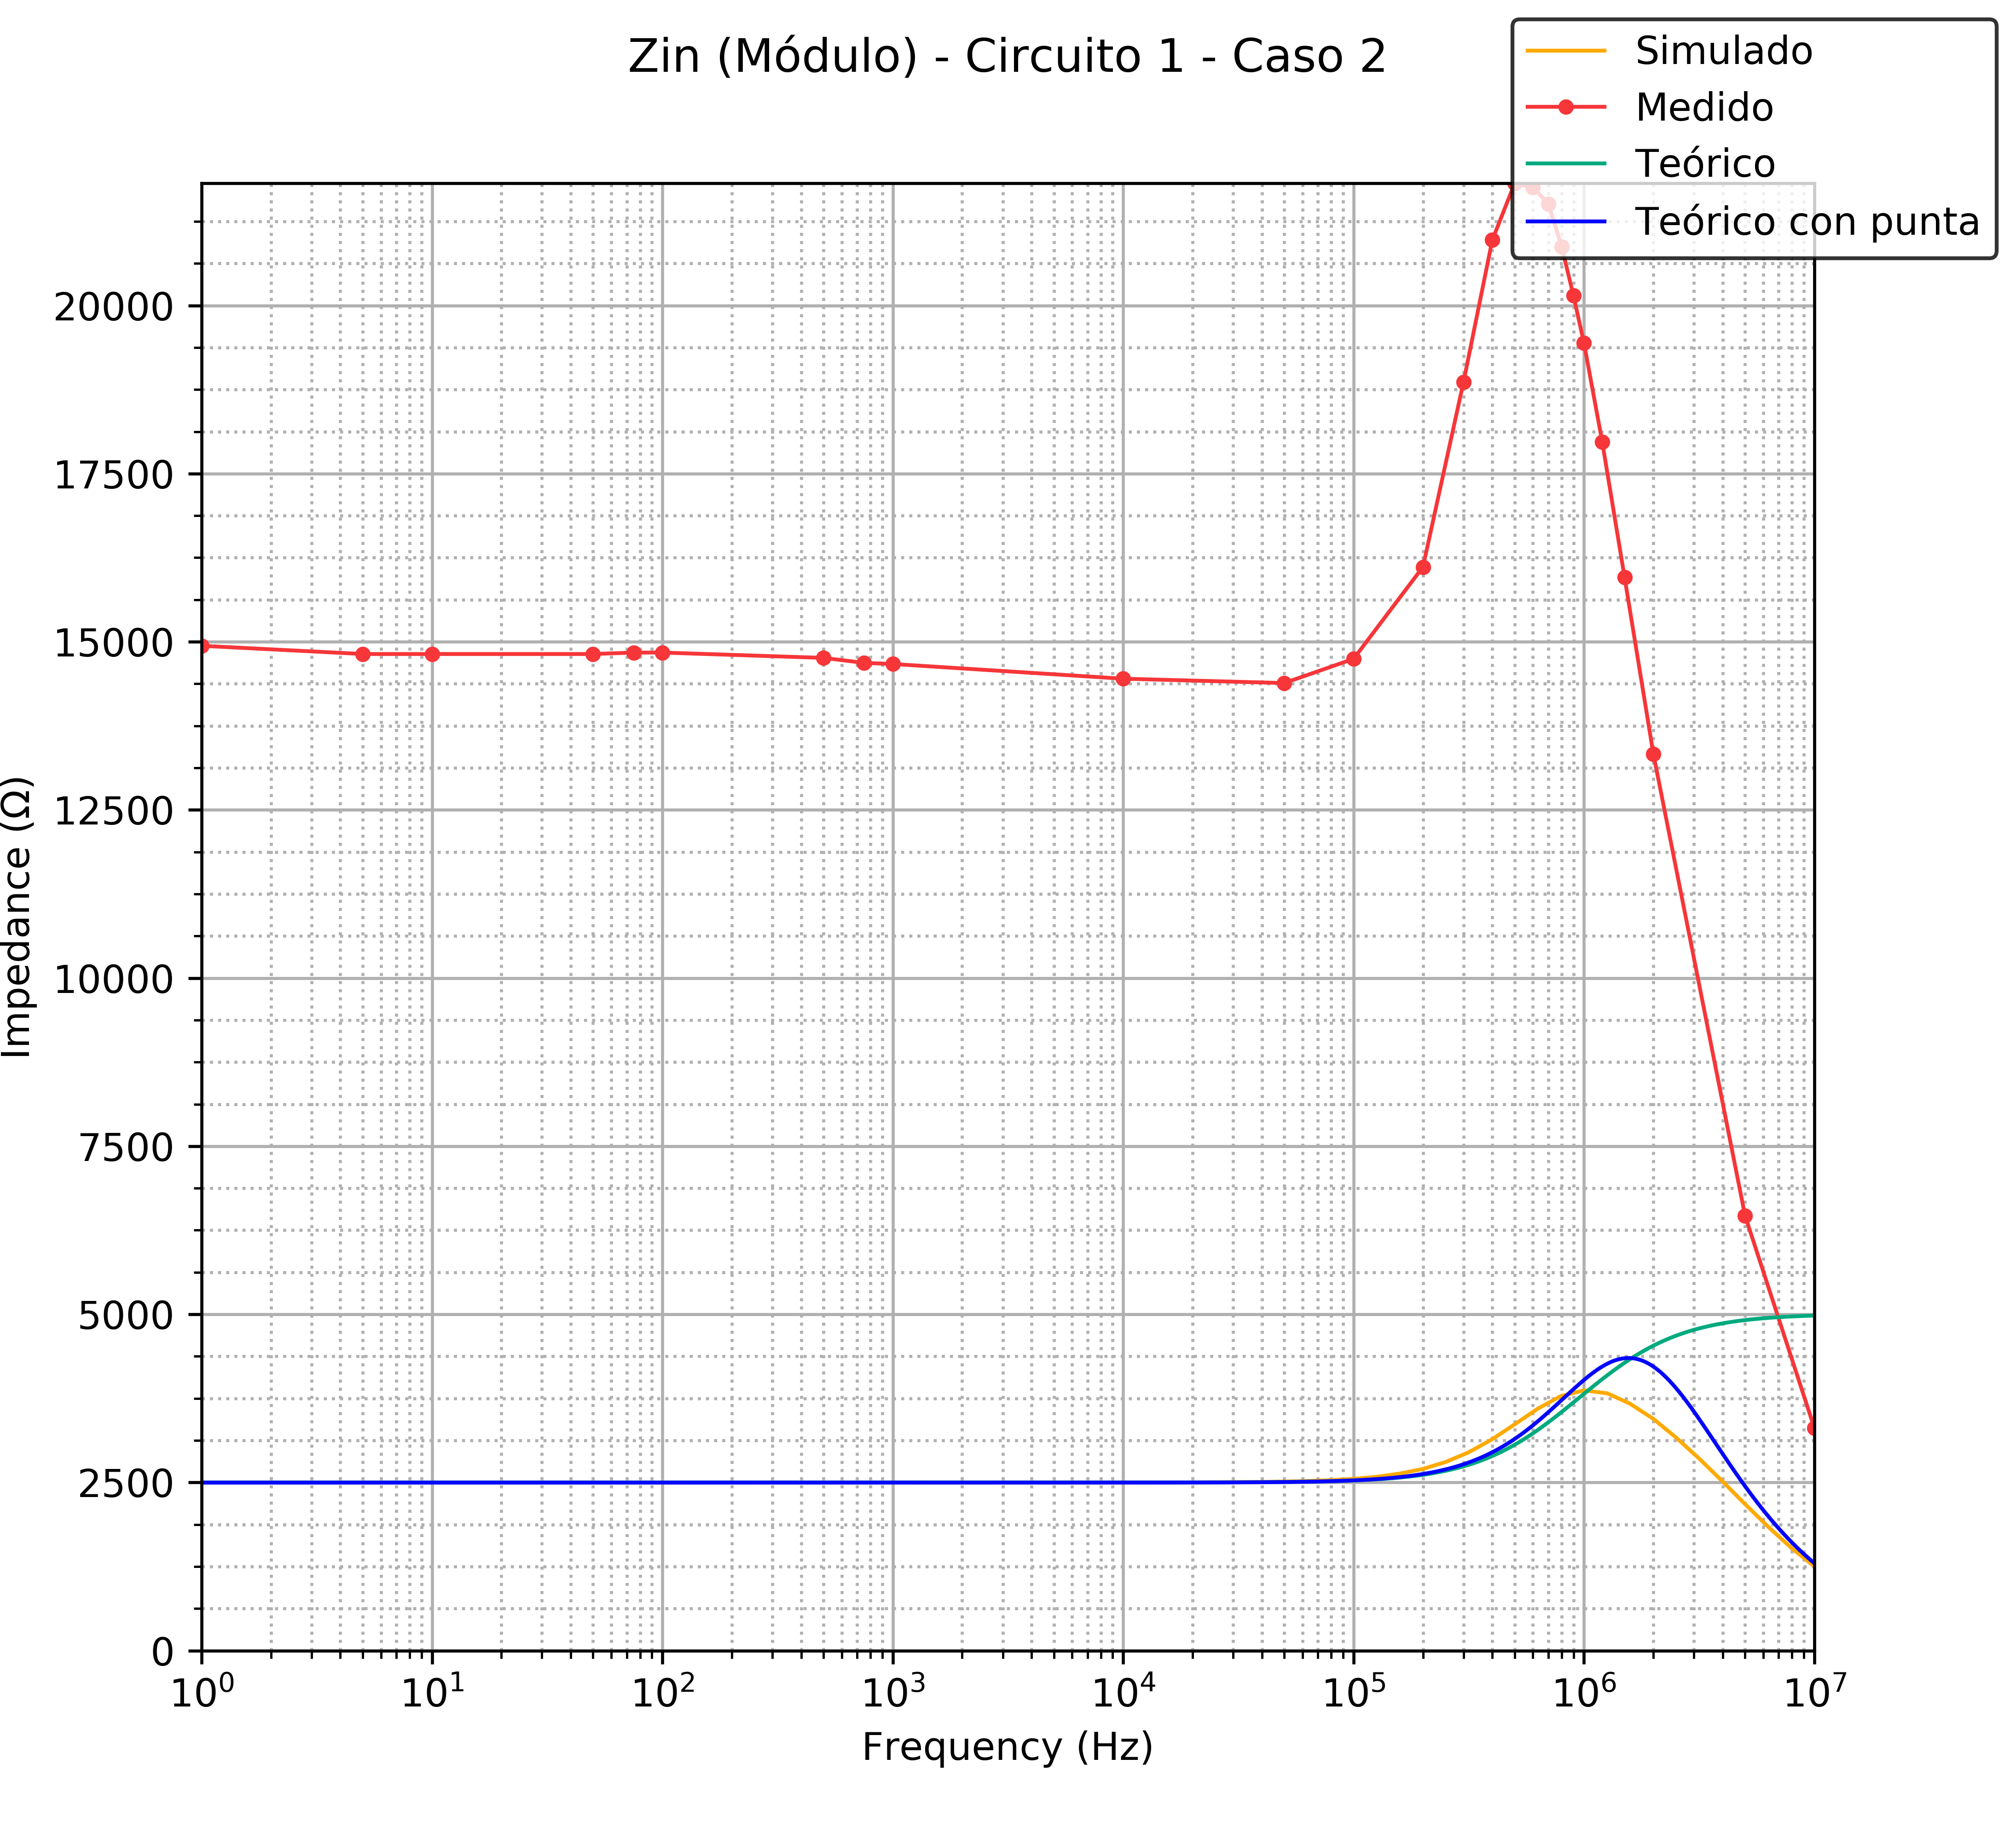
\includegraphics[width=10cm,height=10cm,keepaspectratio]{../EJ1/00GRAFICOS/c1c2/c1c2ZINpunta.png}
	\caption{Configuración inversora - Caso 2 - M\'odulo de $Z_{in}$}
	\label{c1c2zinM}
\end{figure}

\begin{figure}[H] %!ht
	\centering
	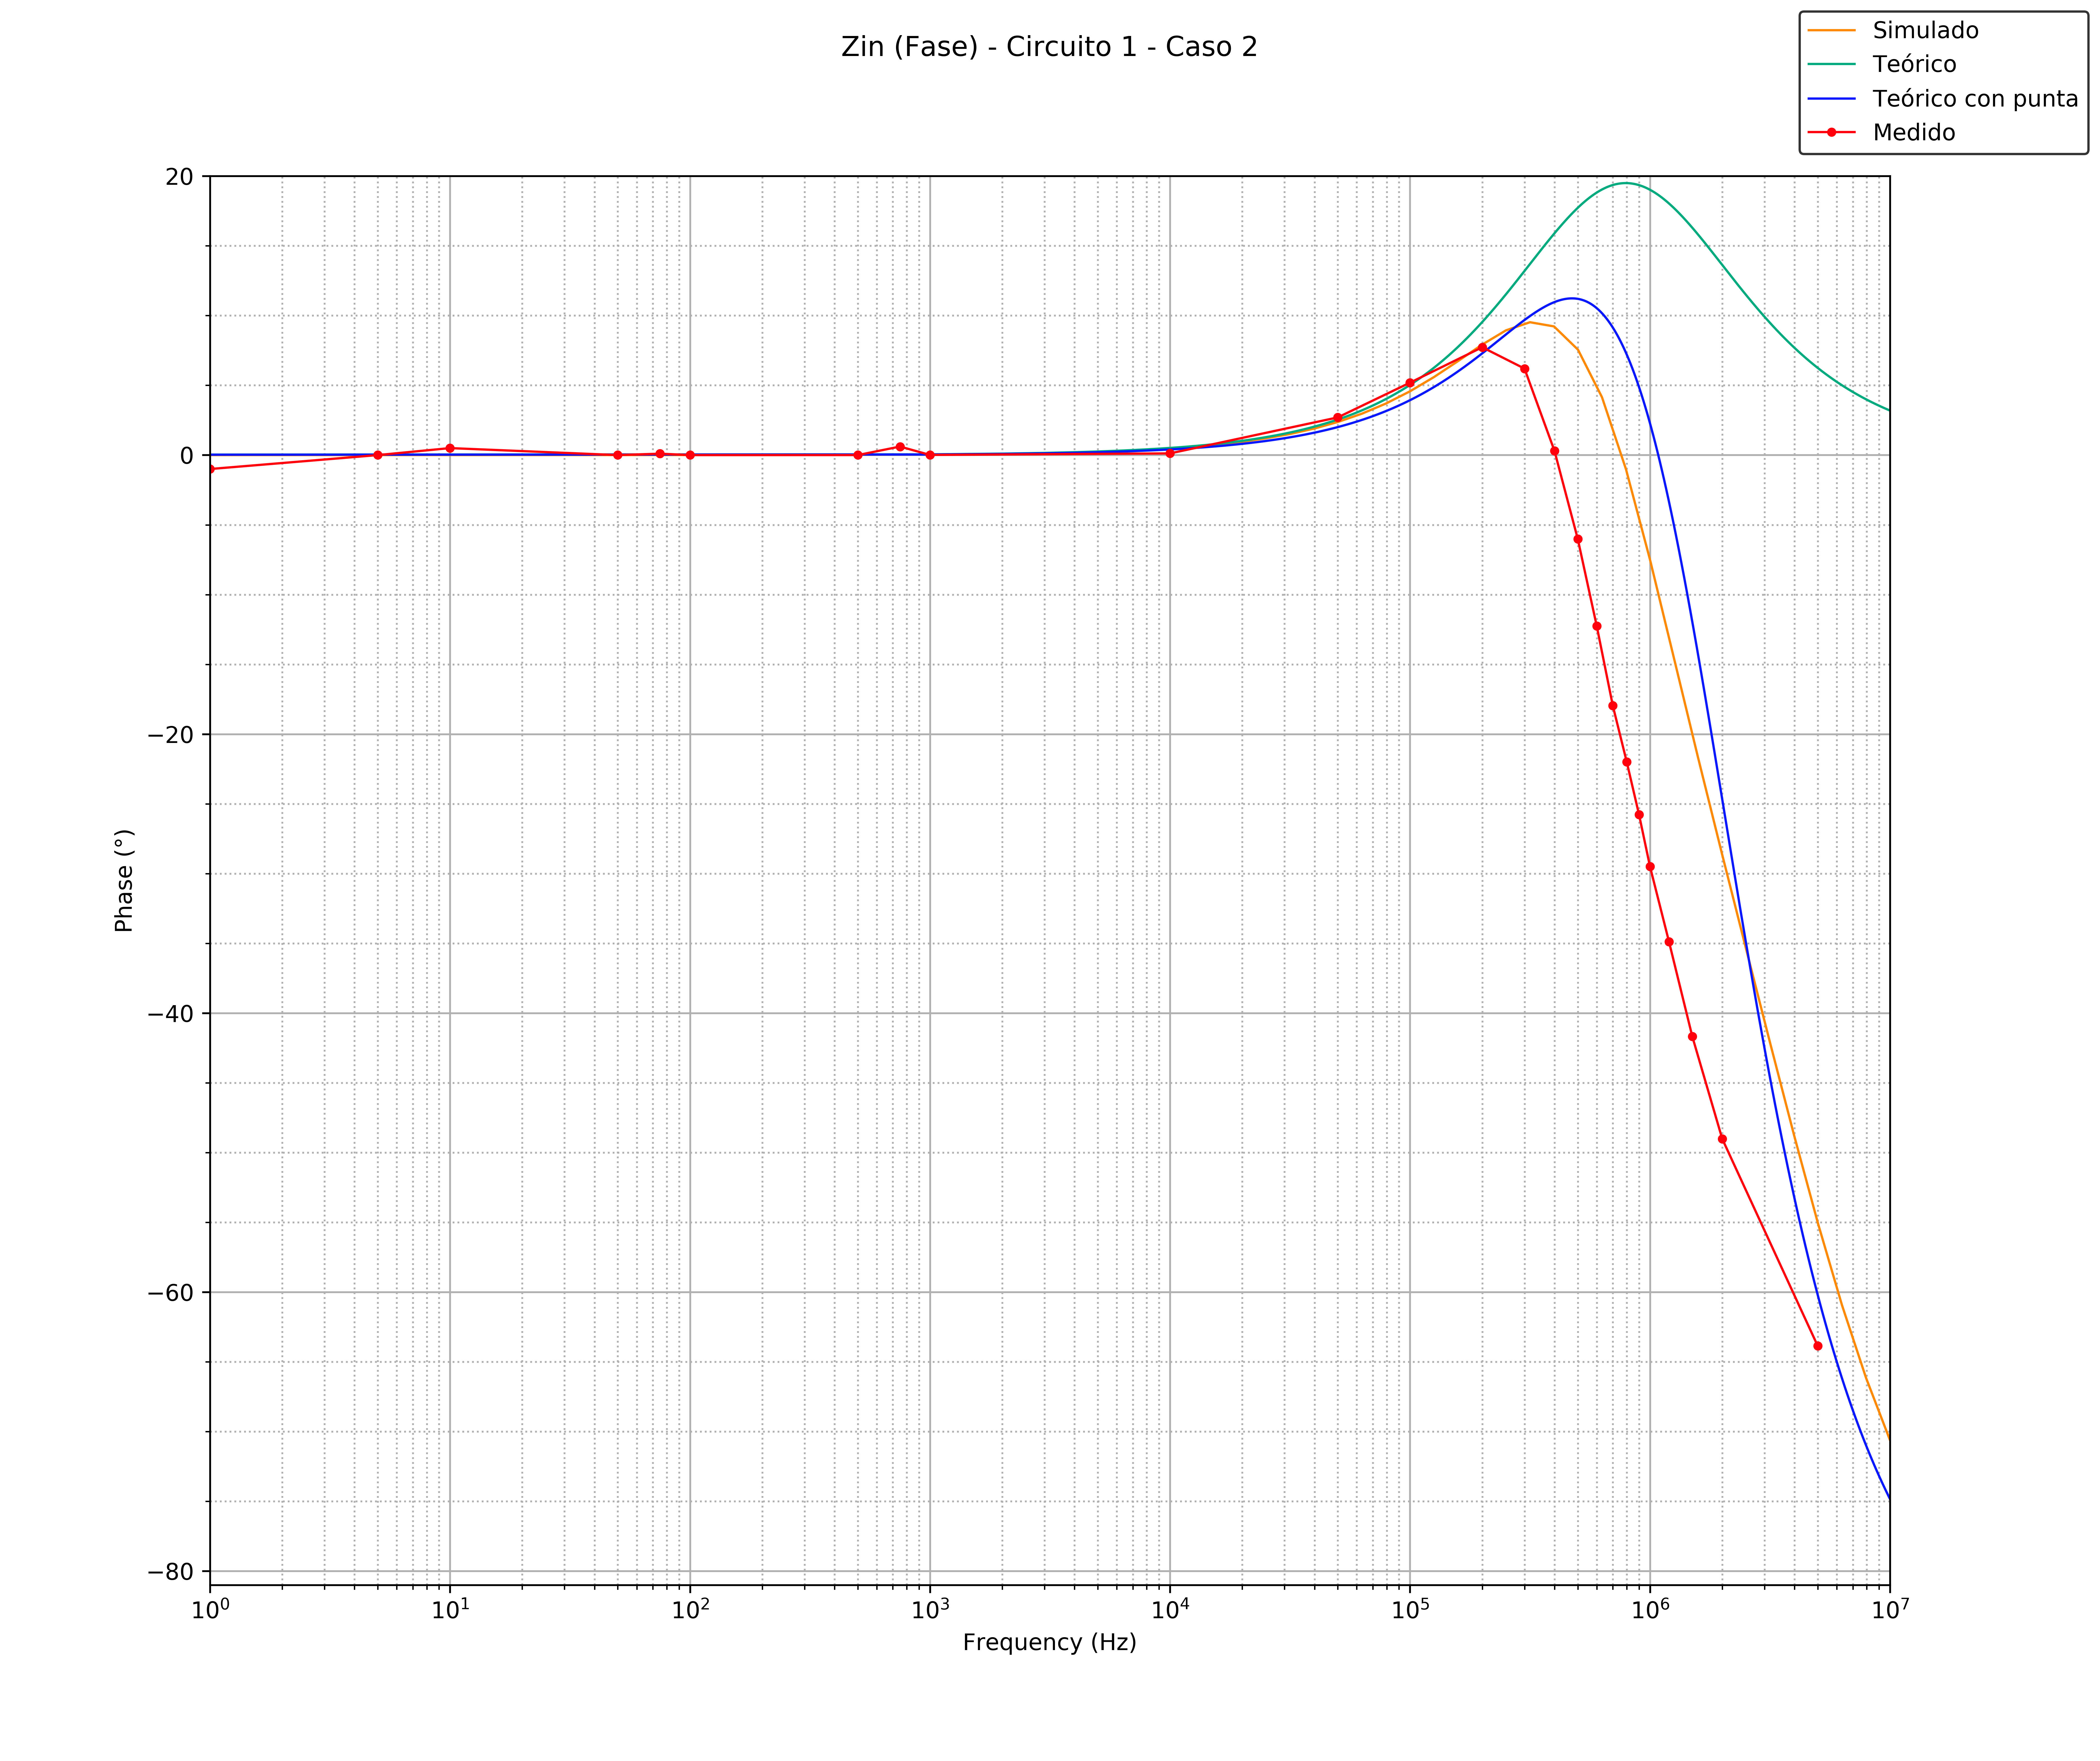
\includegraphics[width=10cm,height=10cm,keepaspectratio]{../EJ1/00GRAFICOS/c1c2/c1c2zinFASE.png}
	\caption{Configuración inversora - Caso 2 - Fase de $Z_{in}$}
	\label{c1c2zinP}
\end{figure}

\begin{figure}[H] %!ht
	\centering
	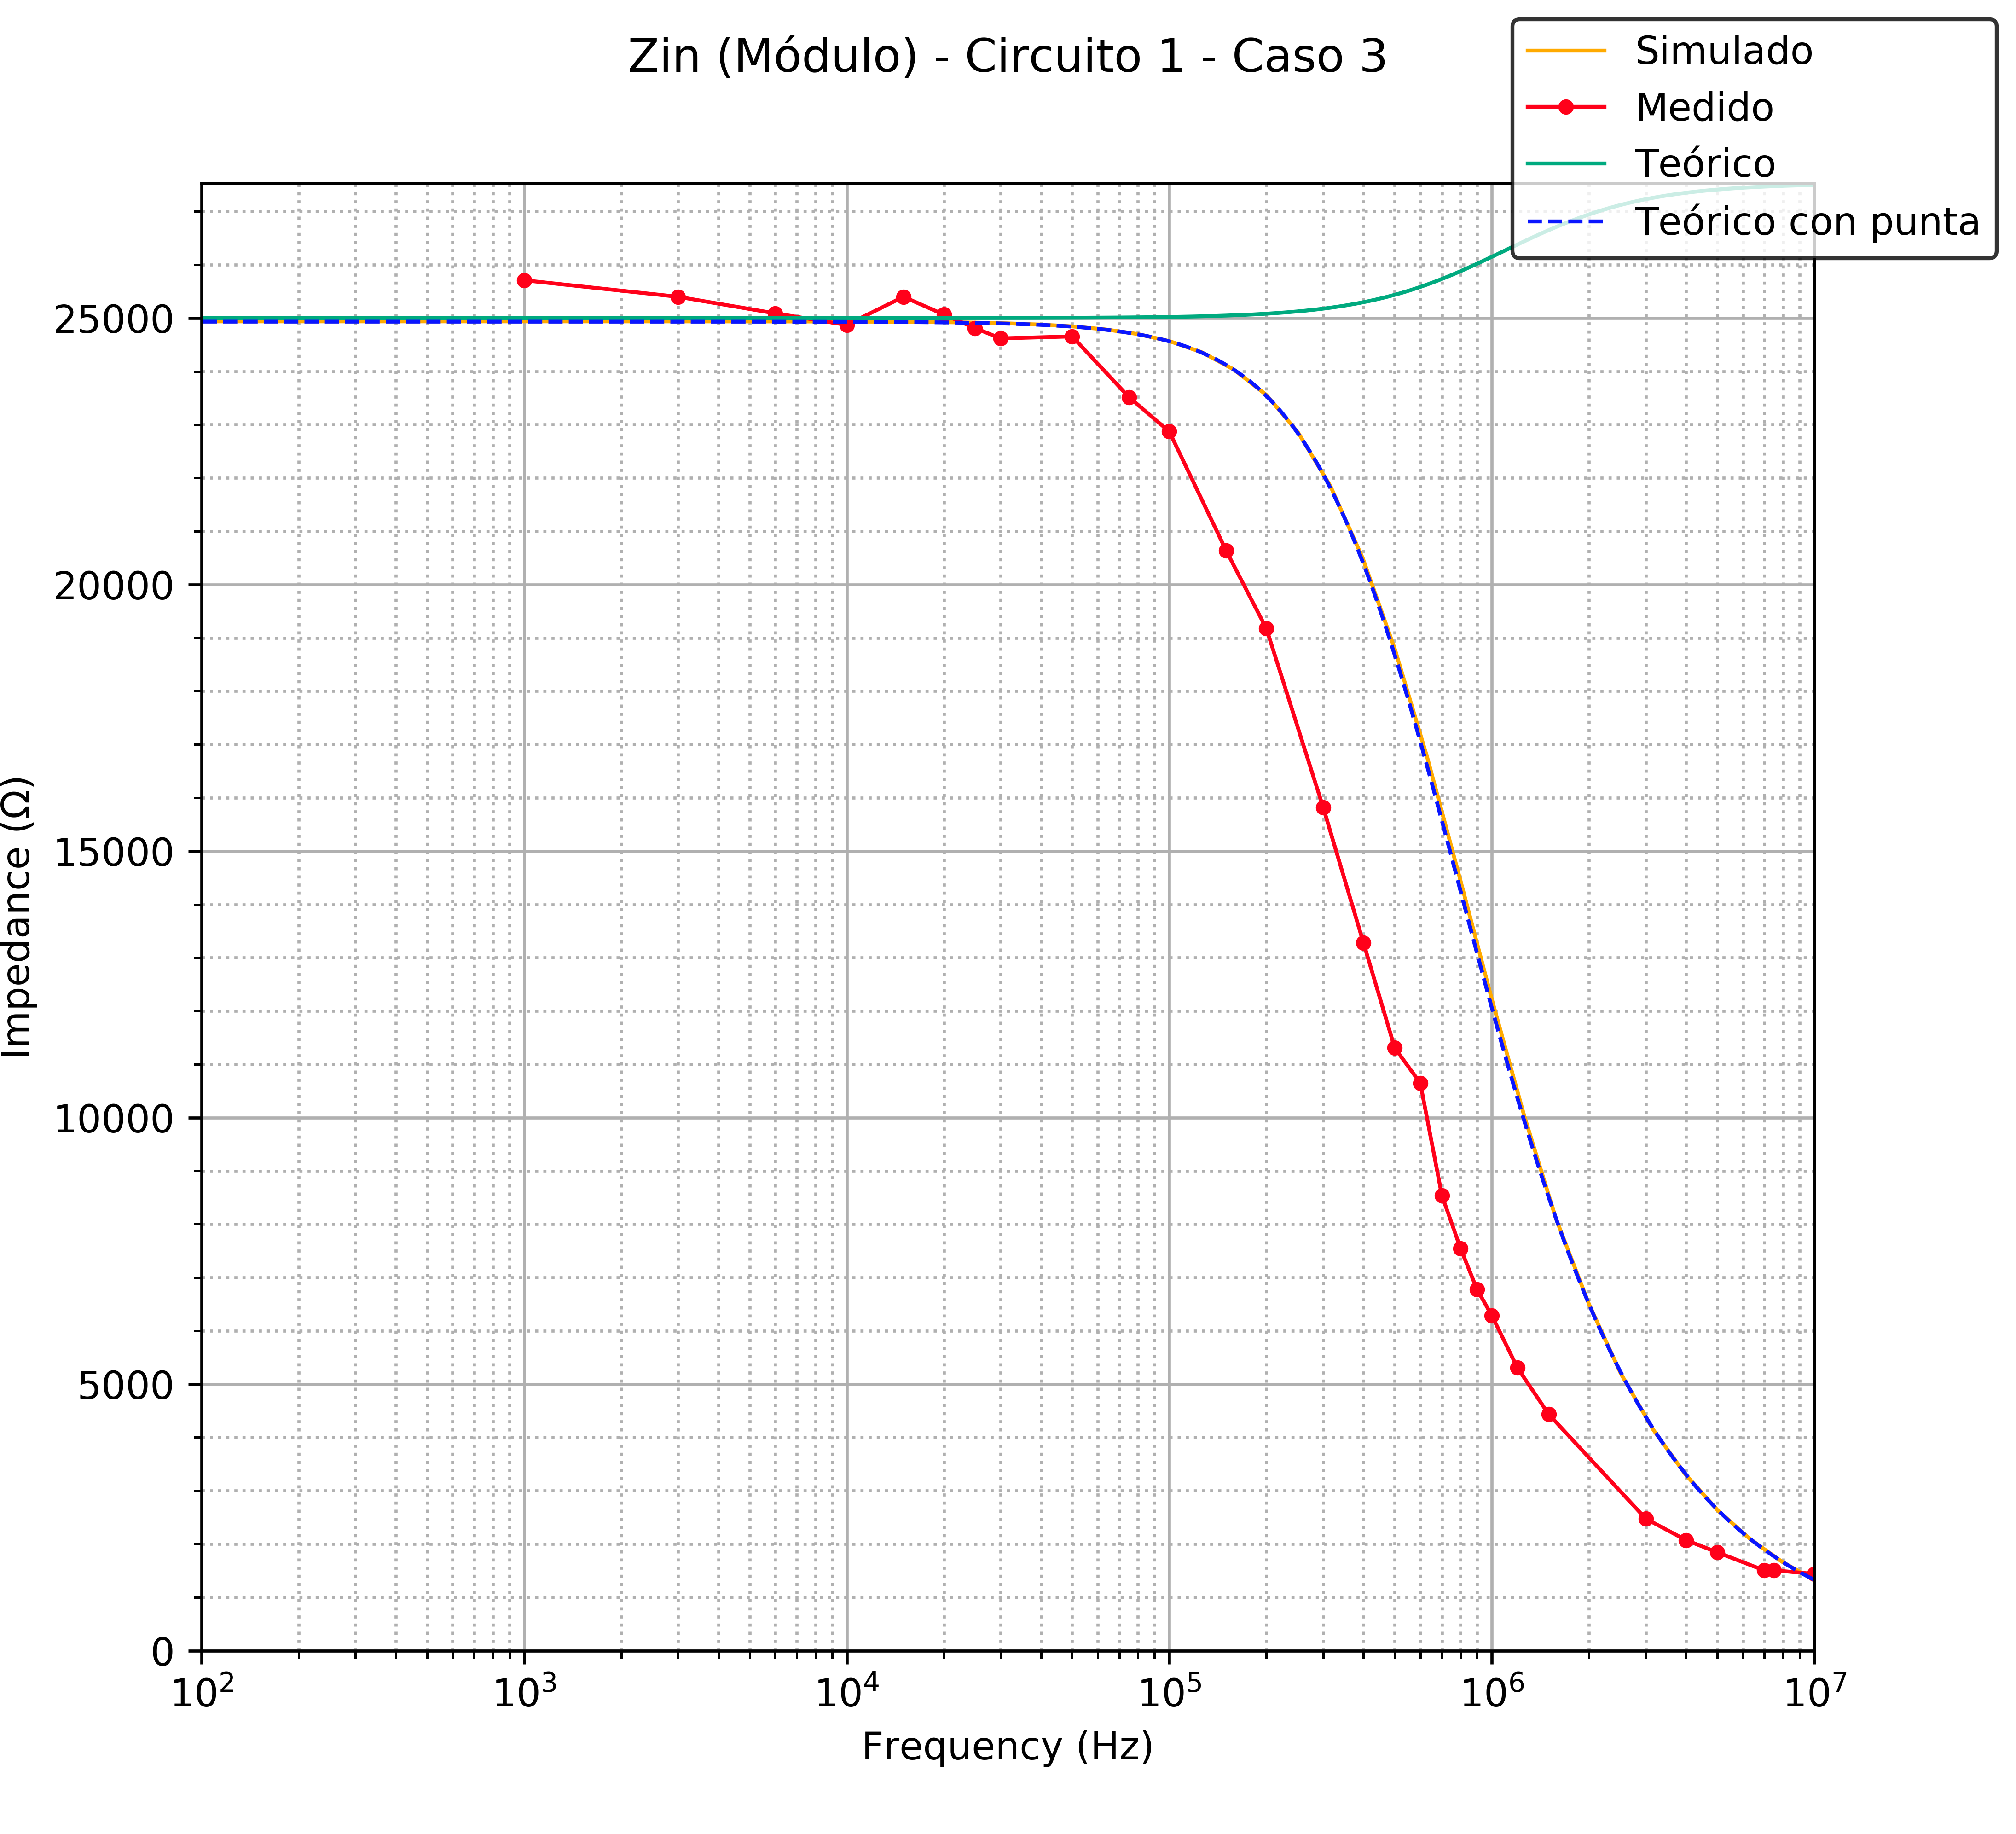
\includegraphics[width=10cm,height=10cm,keepaspectratio]{../EJ1/00GRAFICOS/c1c3/c1c3ZINpunta.png}
	\caption{Configuración inversora - Caso 3 - M\'odulo de $Z_{in}$}
	\label{c1c3zinM}
\end{figure}

\begin{figure}[H] %!ht
	\centering
	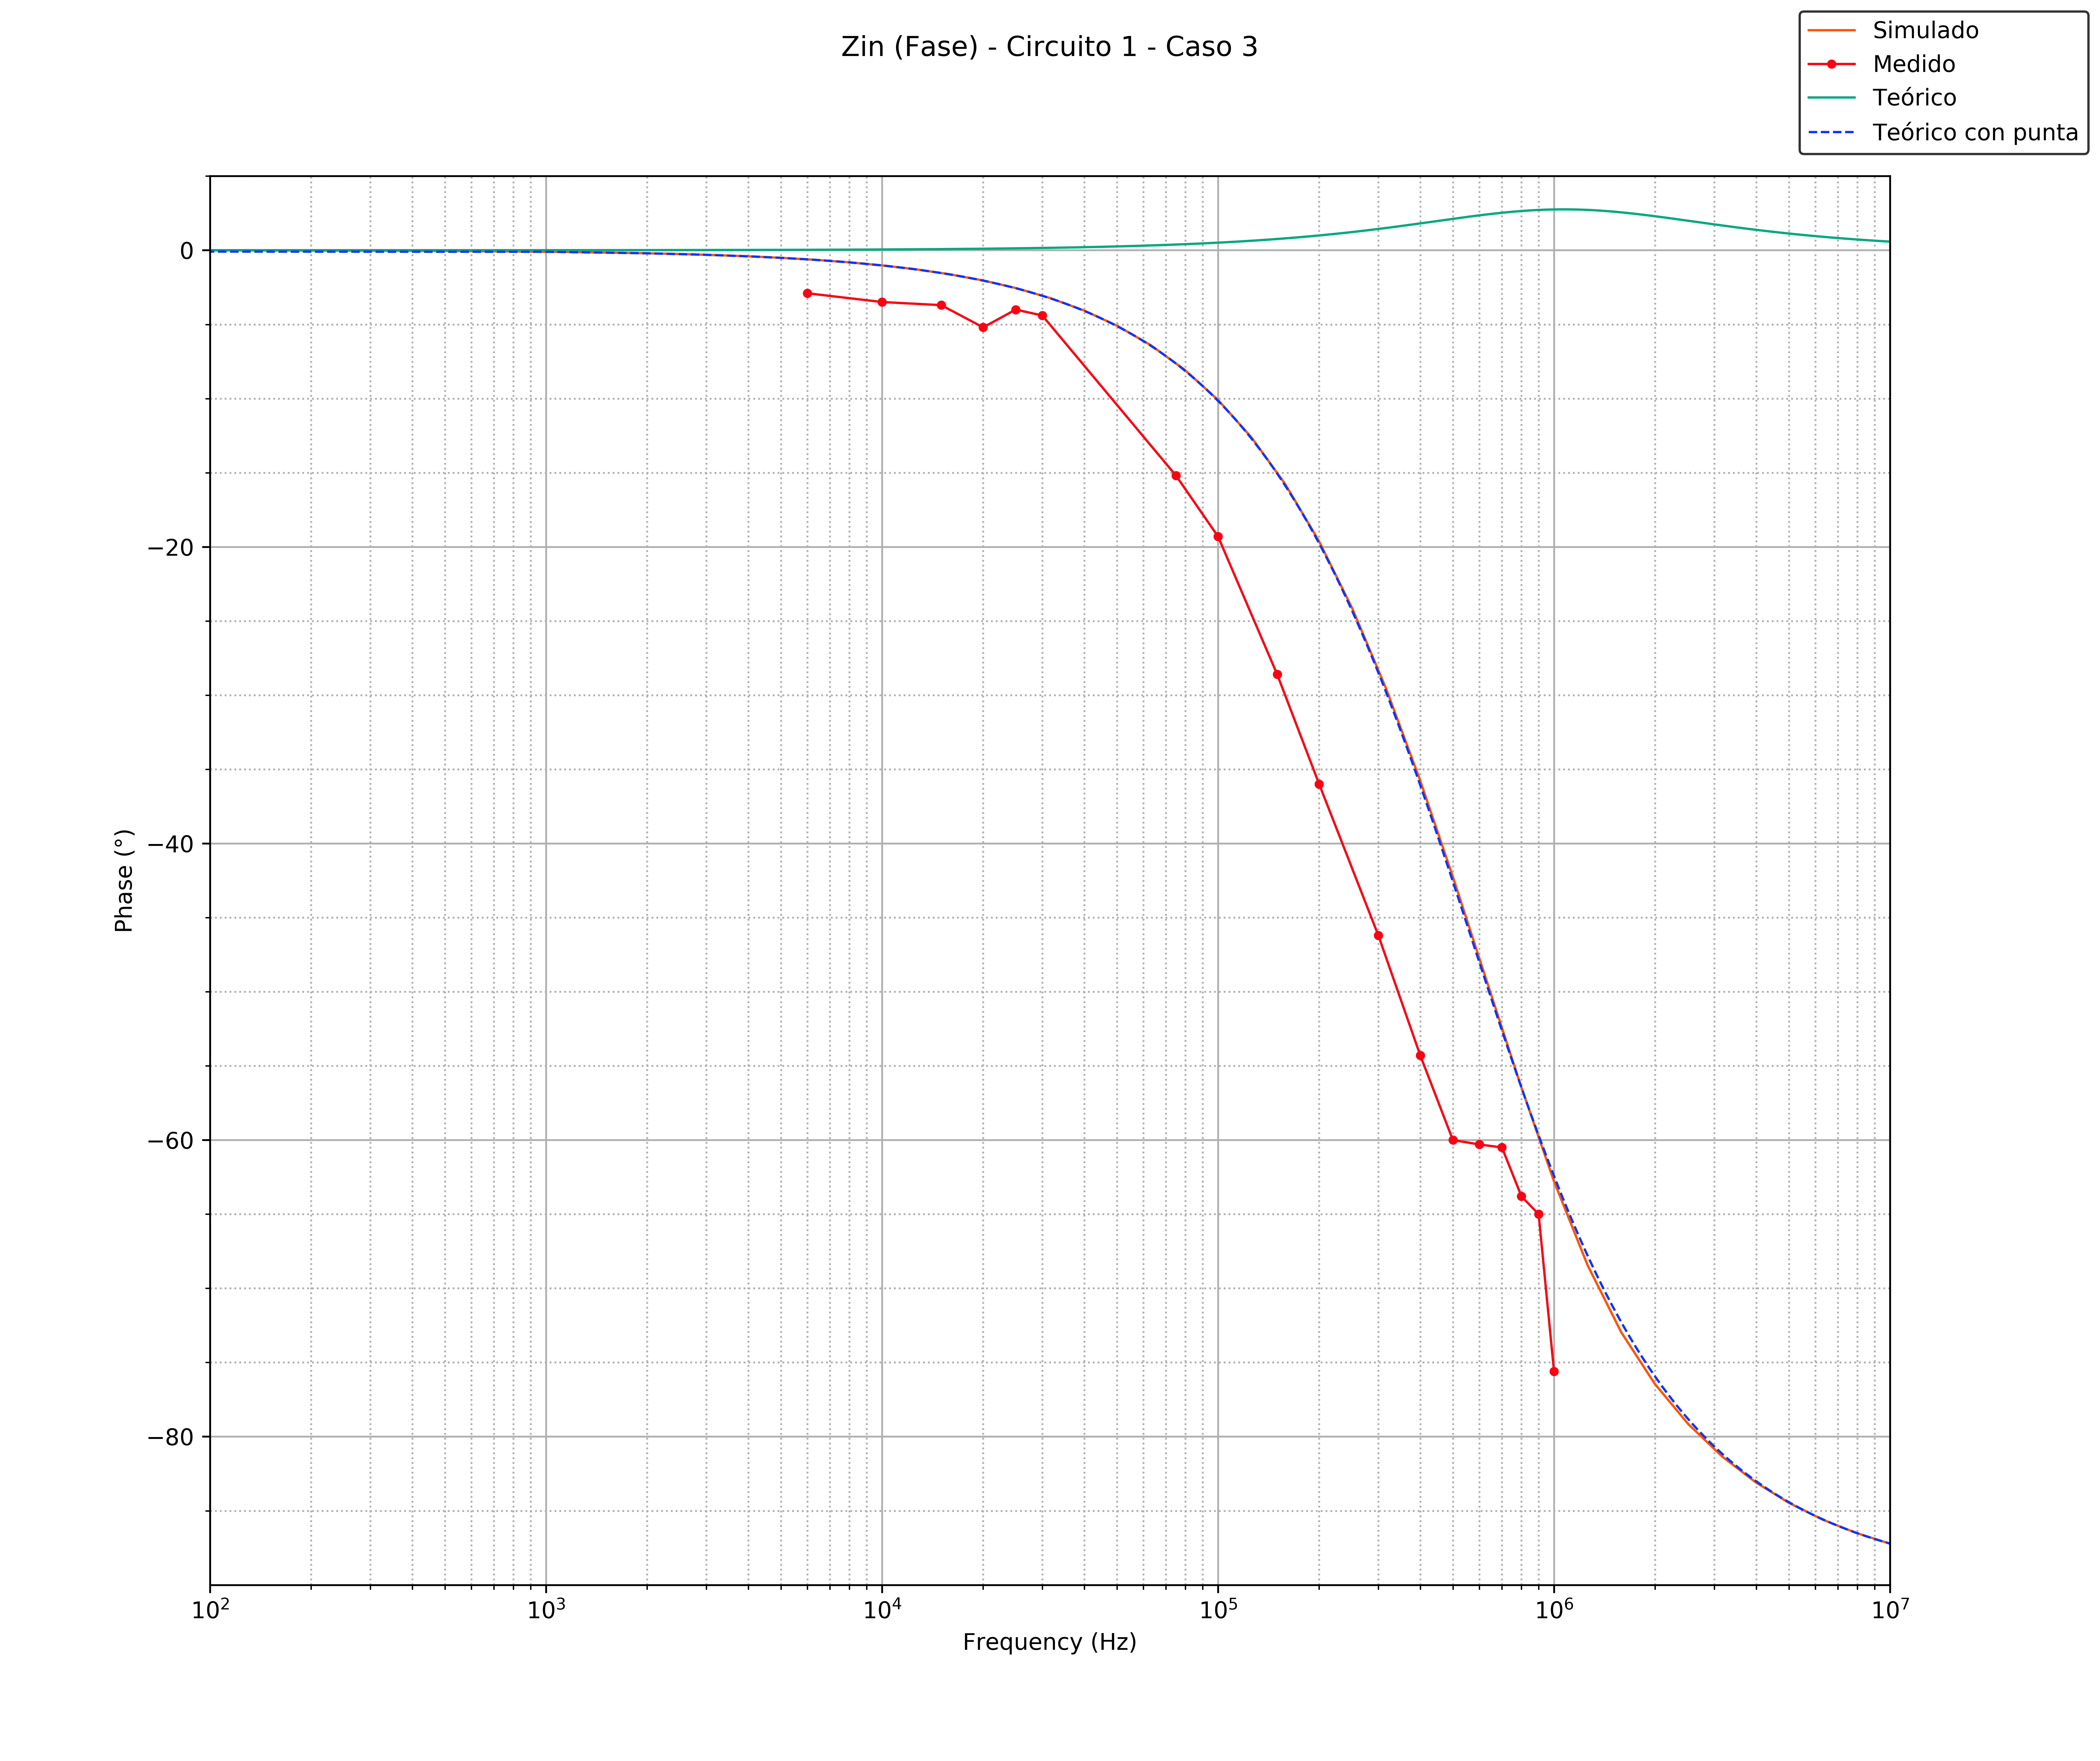
\includegraphics[width=10cm,height=10cm,keepaspectratio]{../EJ1/00GRAFICOS/c1c3/c1c3zinFASE.png}
	\caption{Configuración inversora - Caso 3 - Fase de $Z_{in}$}
	\label{c1c3zinP}
\end{figure}

\subsubsection*{Configuraci\'on no inversora}
\begin{figure}[H] %!ht
	\centering
	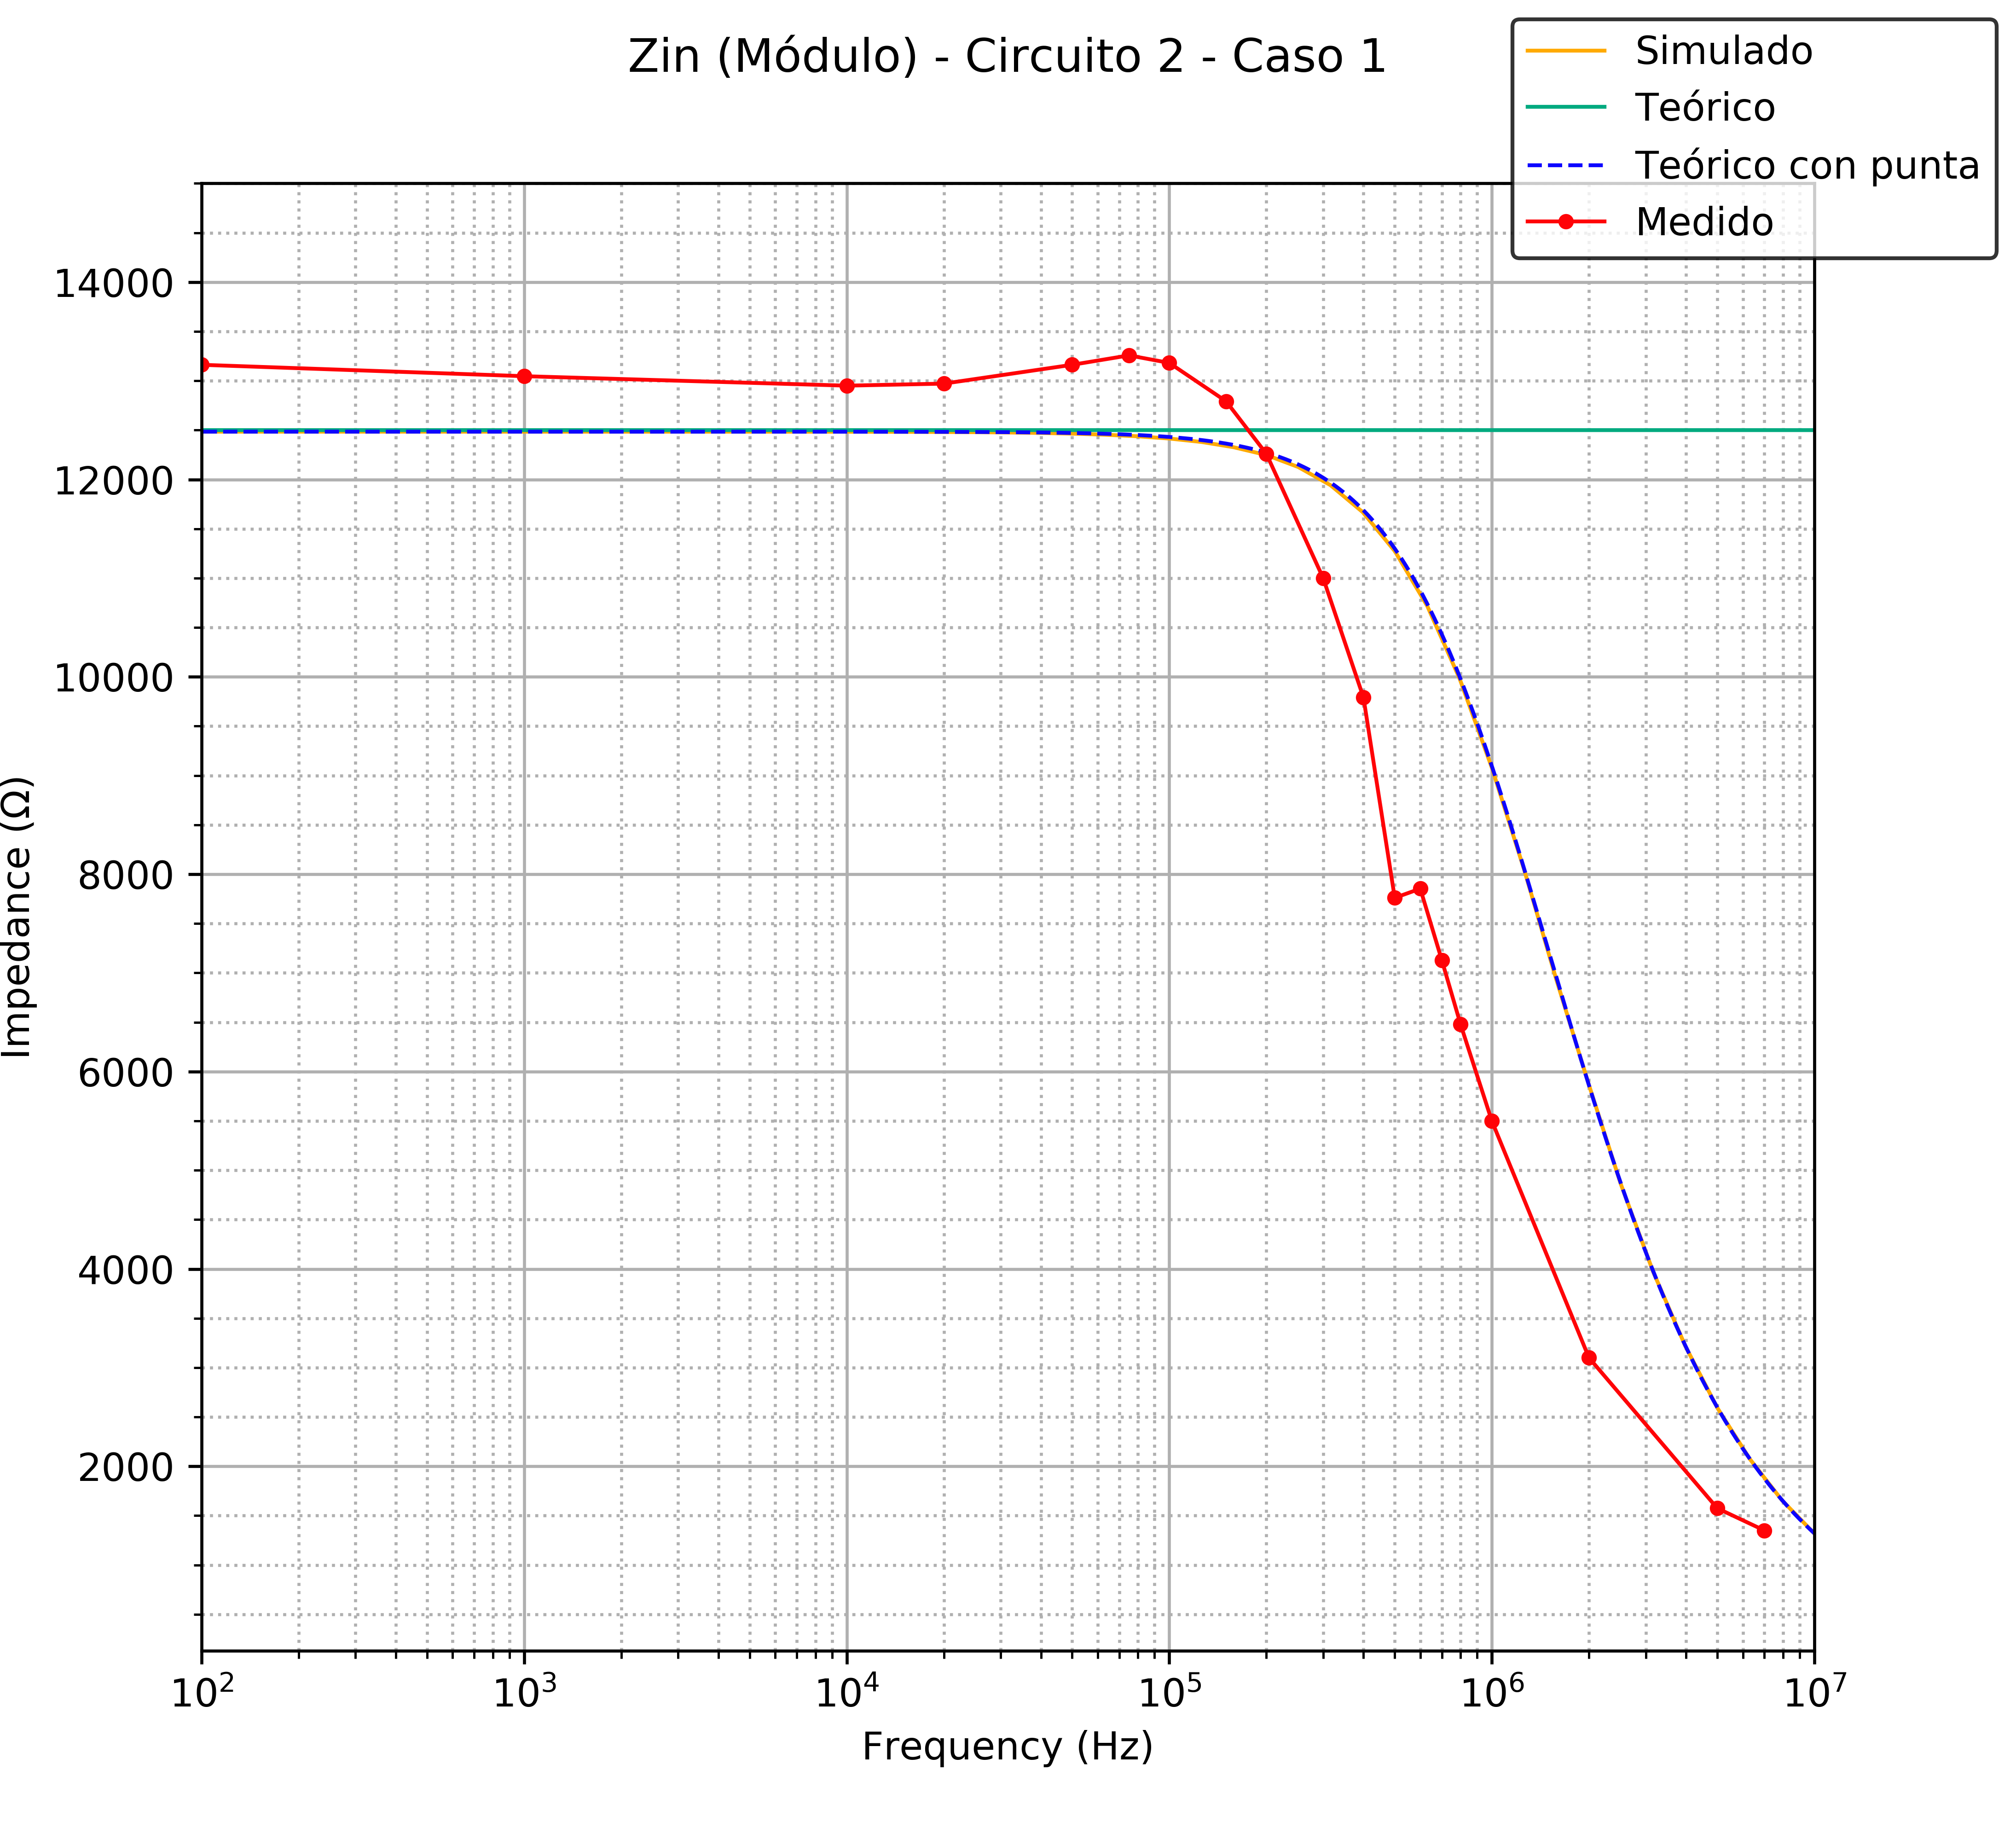
\includegraphics[width=10cm,height=10cm,keepaspectratio]{../EJ1/00GRAFICOS/c2c1/c2c1ZINpunta.png}
	\caption{Configuración no inversora - Caso 1 - M\'odulo de $Z_{in}$}
	\label{c2c1zinM}
\end{figure}

\begin{figure}[H] %!ht
	\centering
	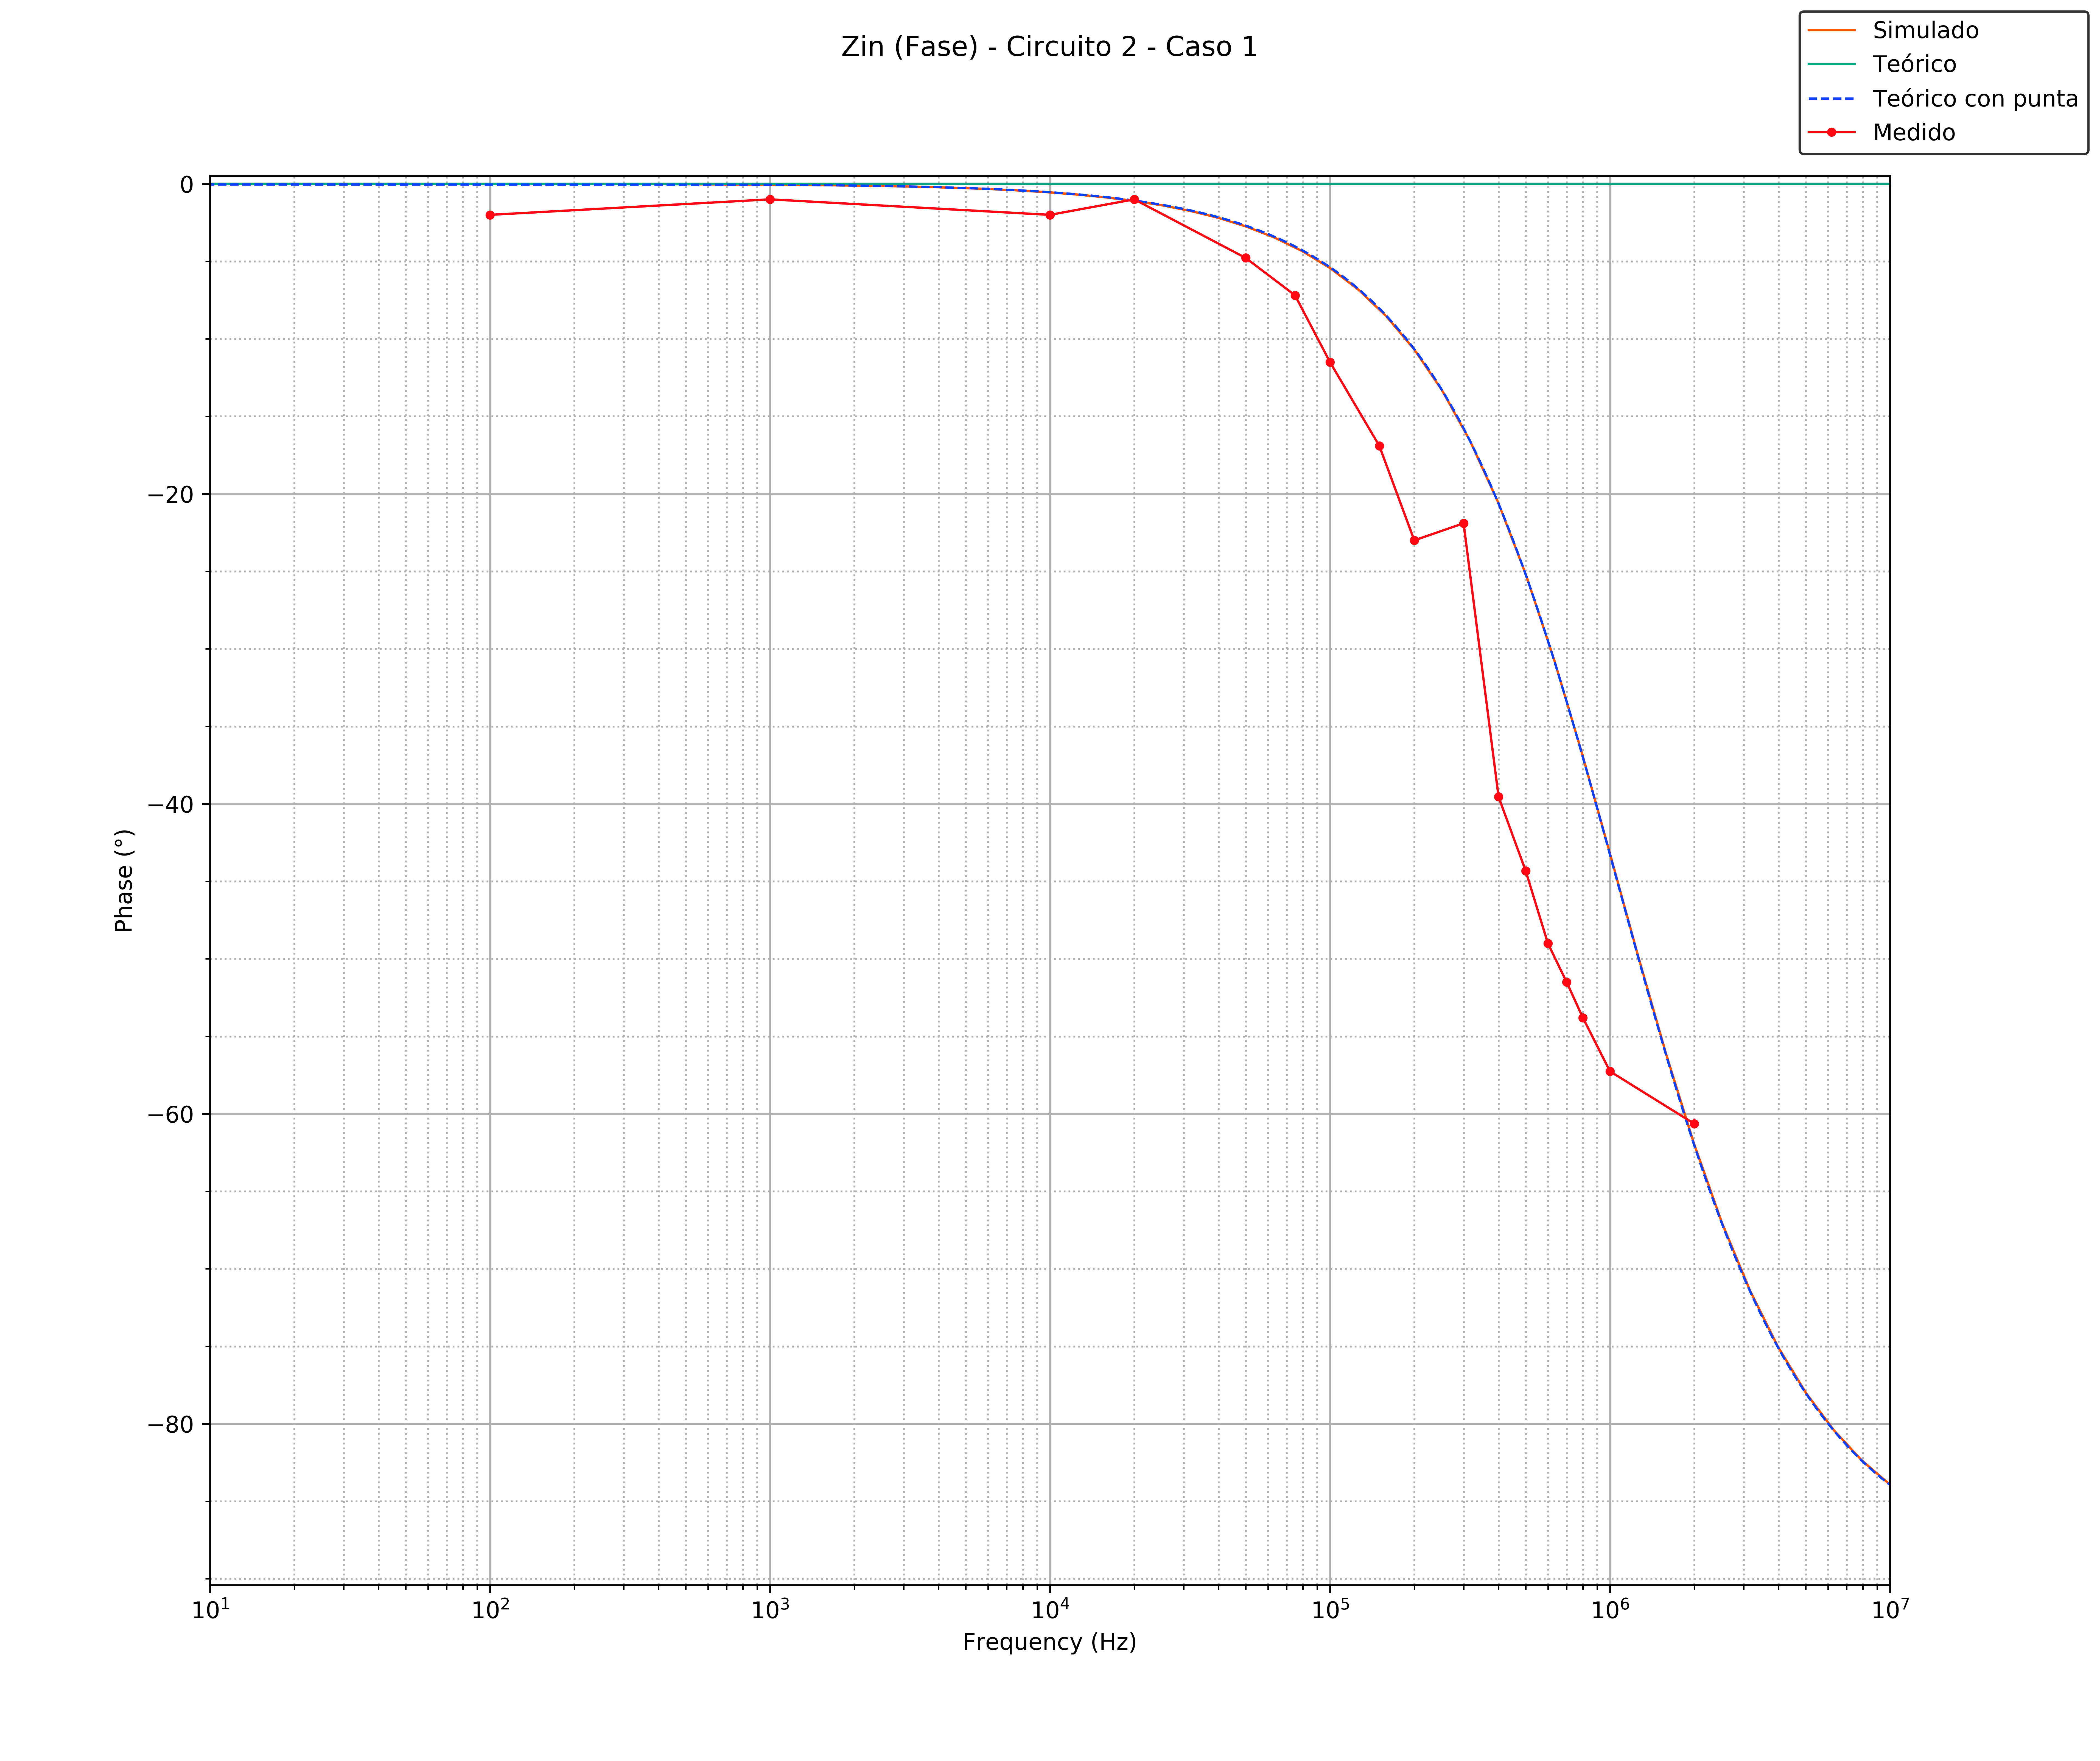
\includegraphics[width=10cm,height=10cm,keepaspectratio]{../EJ1/00GRAFICOS/c2c1/c2c1zinFASE.png}
	\caption{Configuración no inversora - Caso 1 - Fase de $Z_{in}$}
	\label{c2c1zinP}
\end{figure}

\begin{figure}[H] %!ht
	\centering
	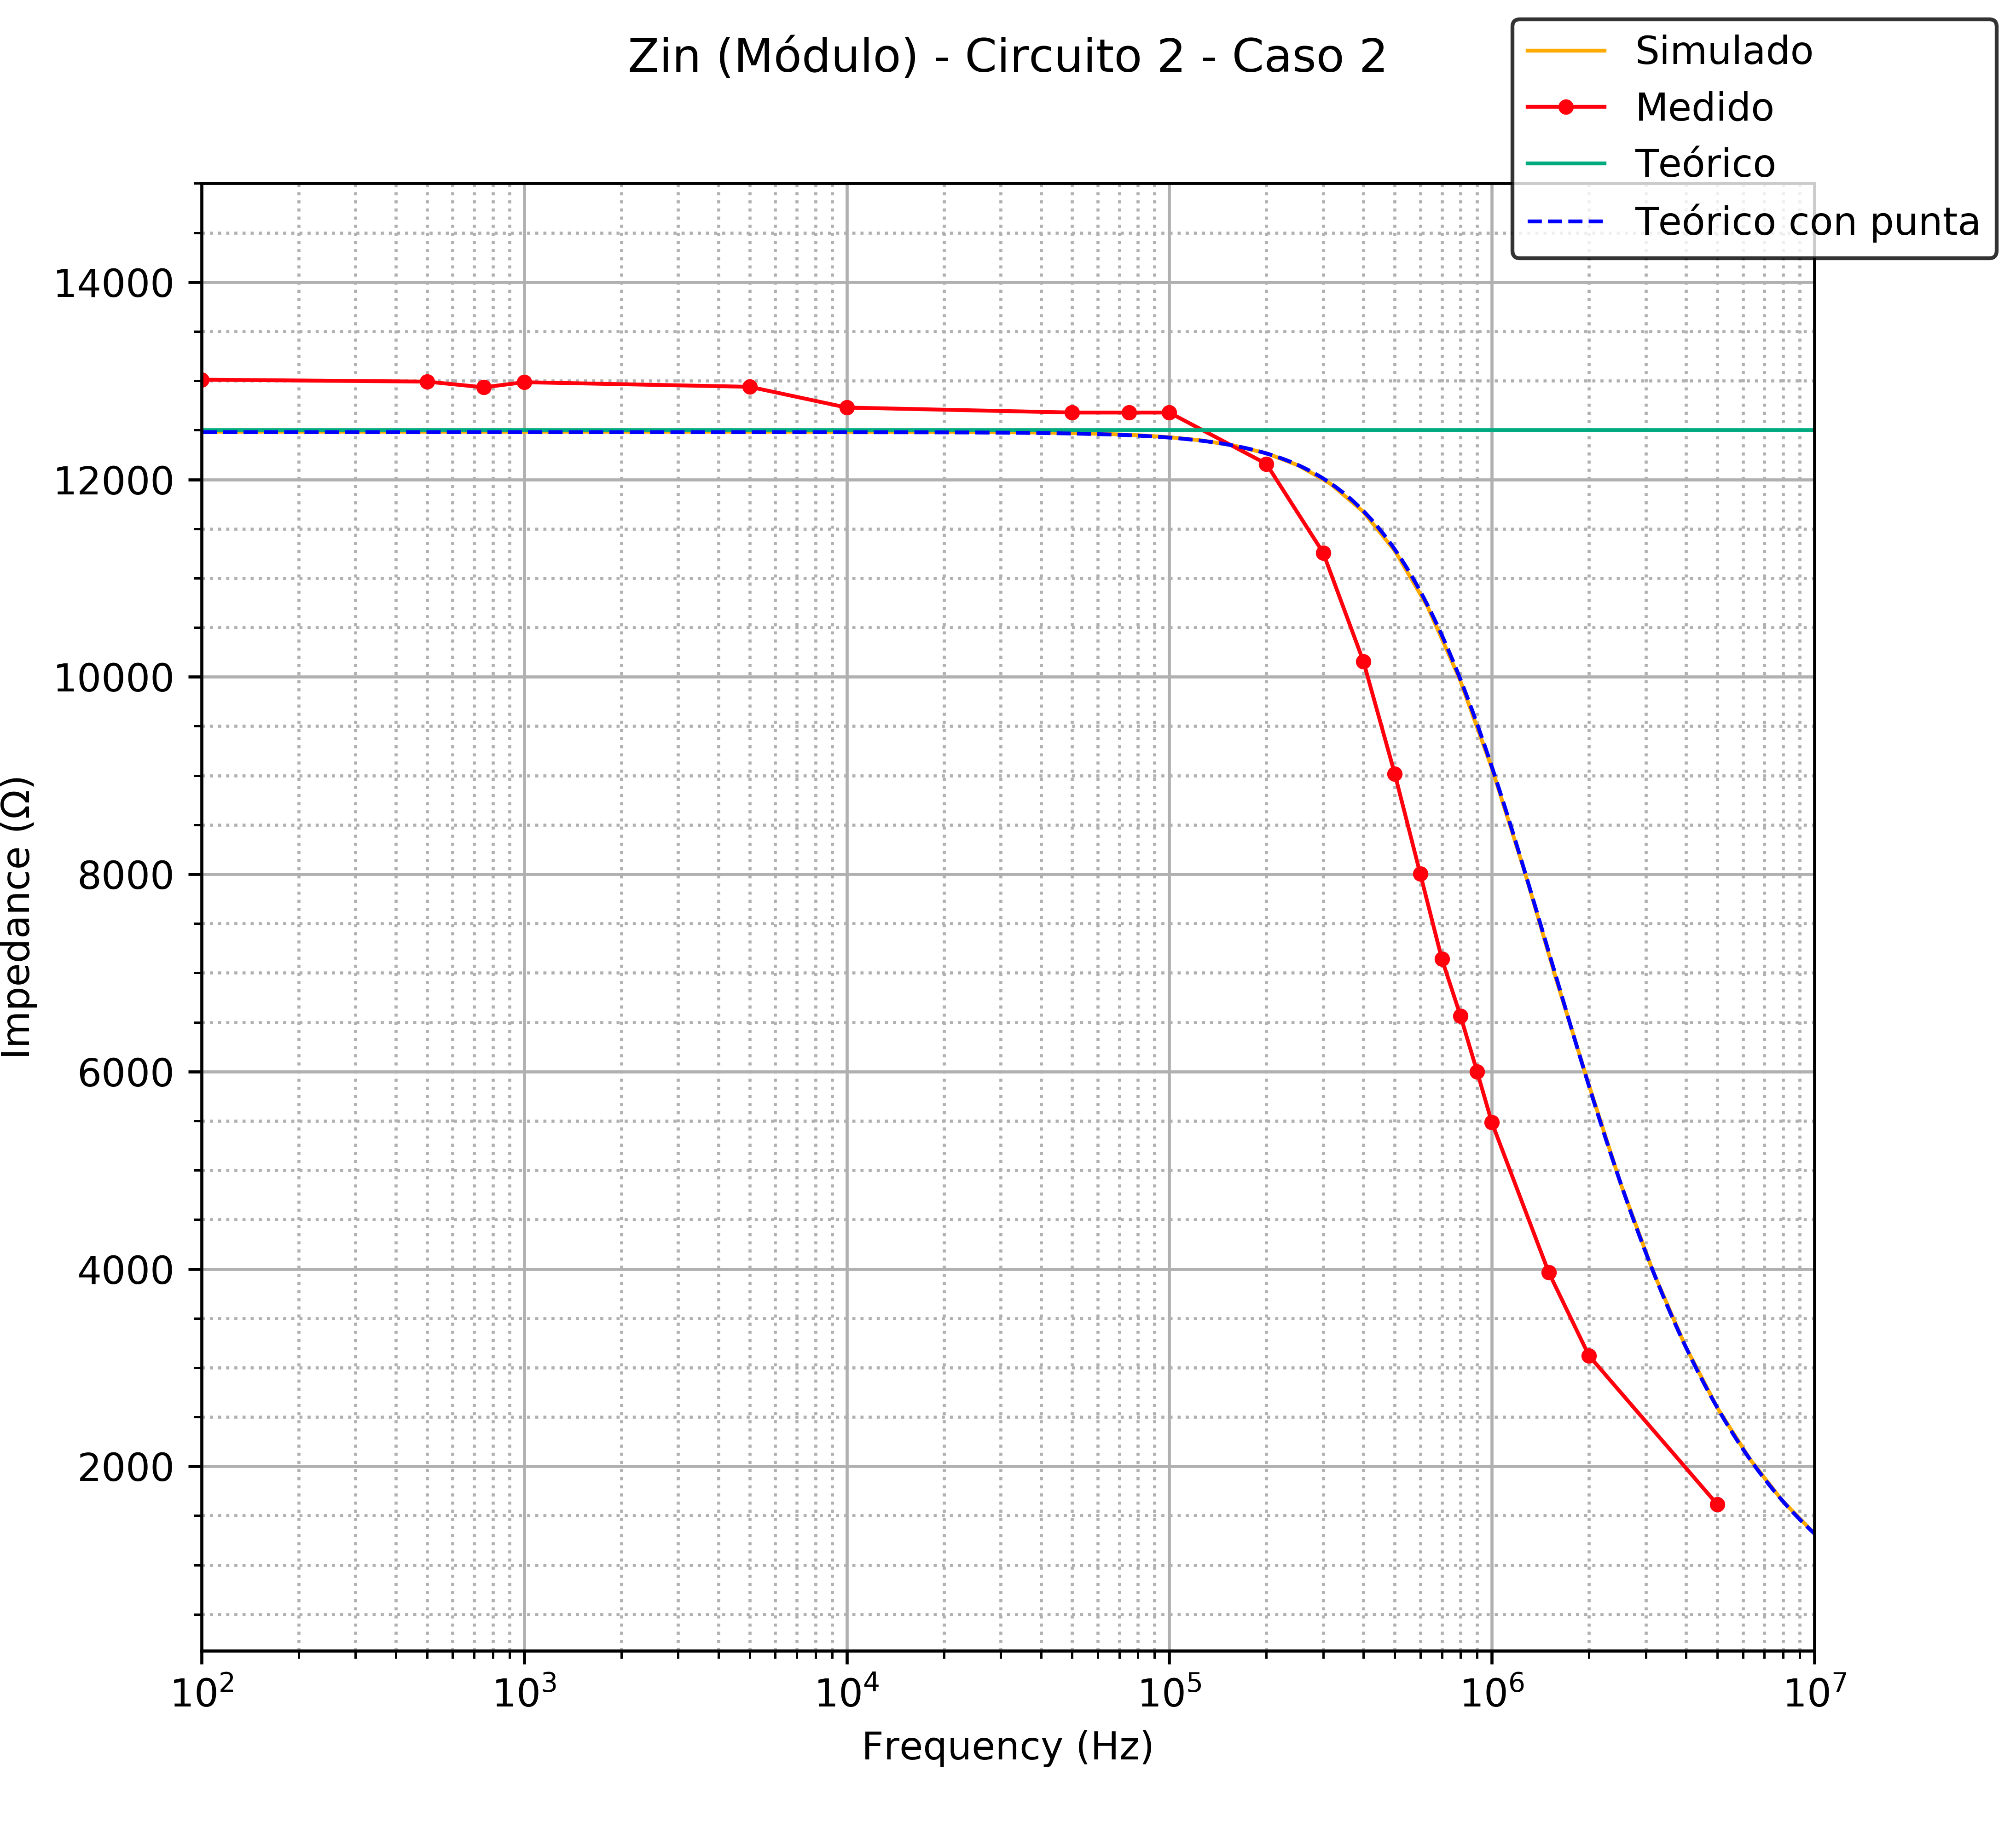
\includegraphics[width=10cm,height=10cm,keepaspectratio]{../EJ1/00GRAFICOS/c2c2/c2c2ZINpunta.png}
	\caption{Configuración no inversora - Caso 2 - M\'odulo de $Z_{in}$}
	\label{c2c2zinM}
\end{figure}

\begin{figure}[H] %!ht
	\centering
	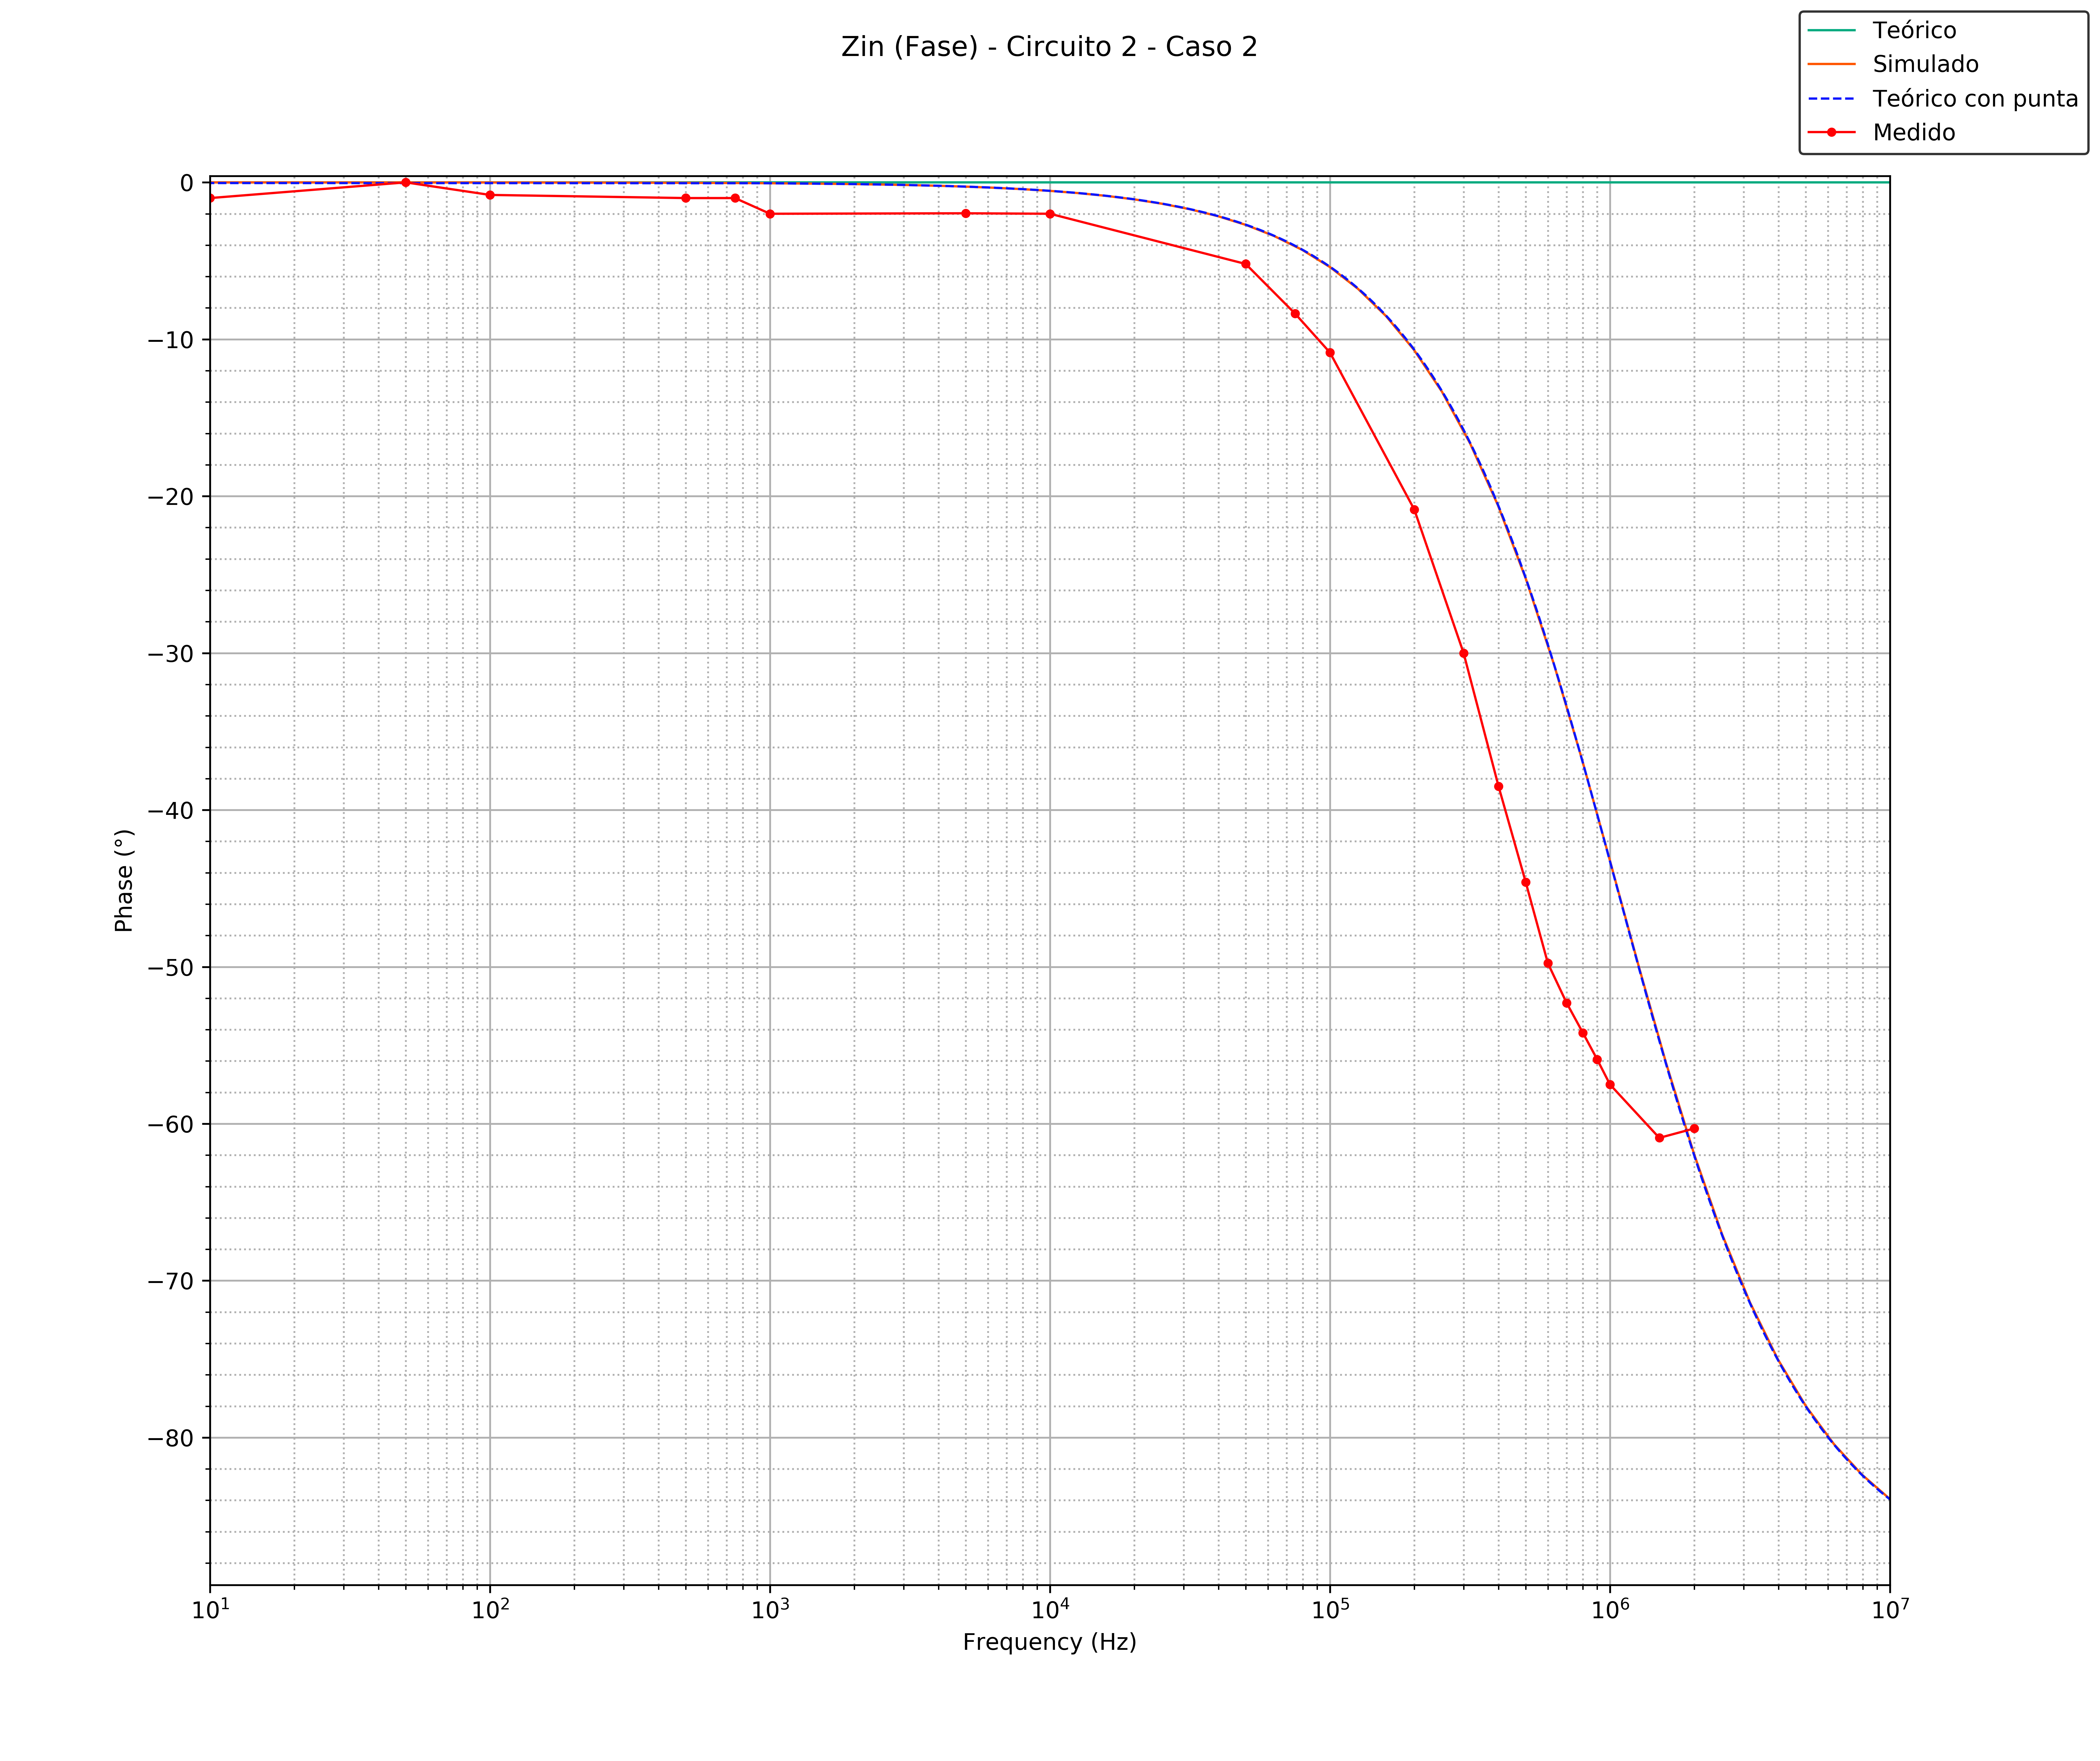
\includegraphics[width=10cm,height=10cm,keepaspectratio]{../EJ1/00GRAFICOS/c2c2/c2c2zinFASE.png}
	\caption{Configuración no inversora - Caso 2 - Fase de $Z_{in}$}
	\label{c2c2zinP}
\end{figure}

%\begin{figure}[H] %!ht
%	\centering
%	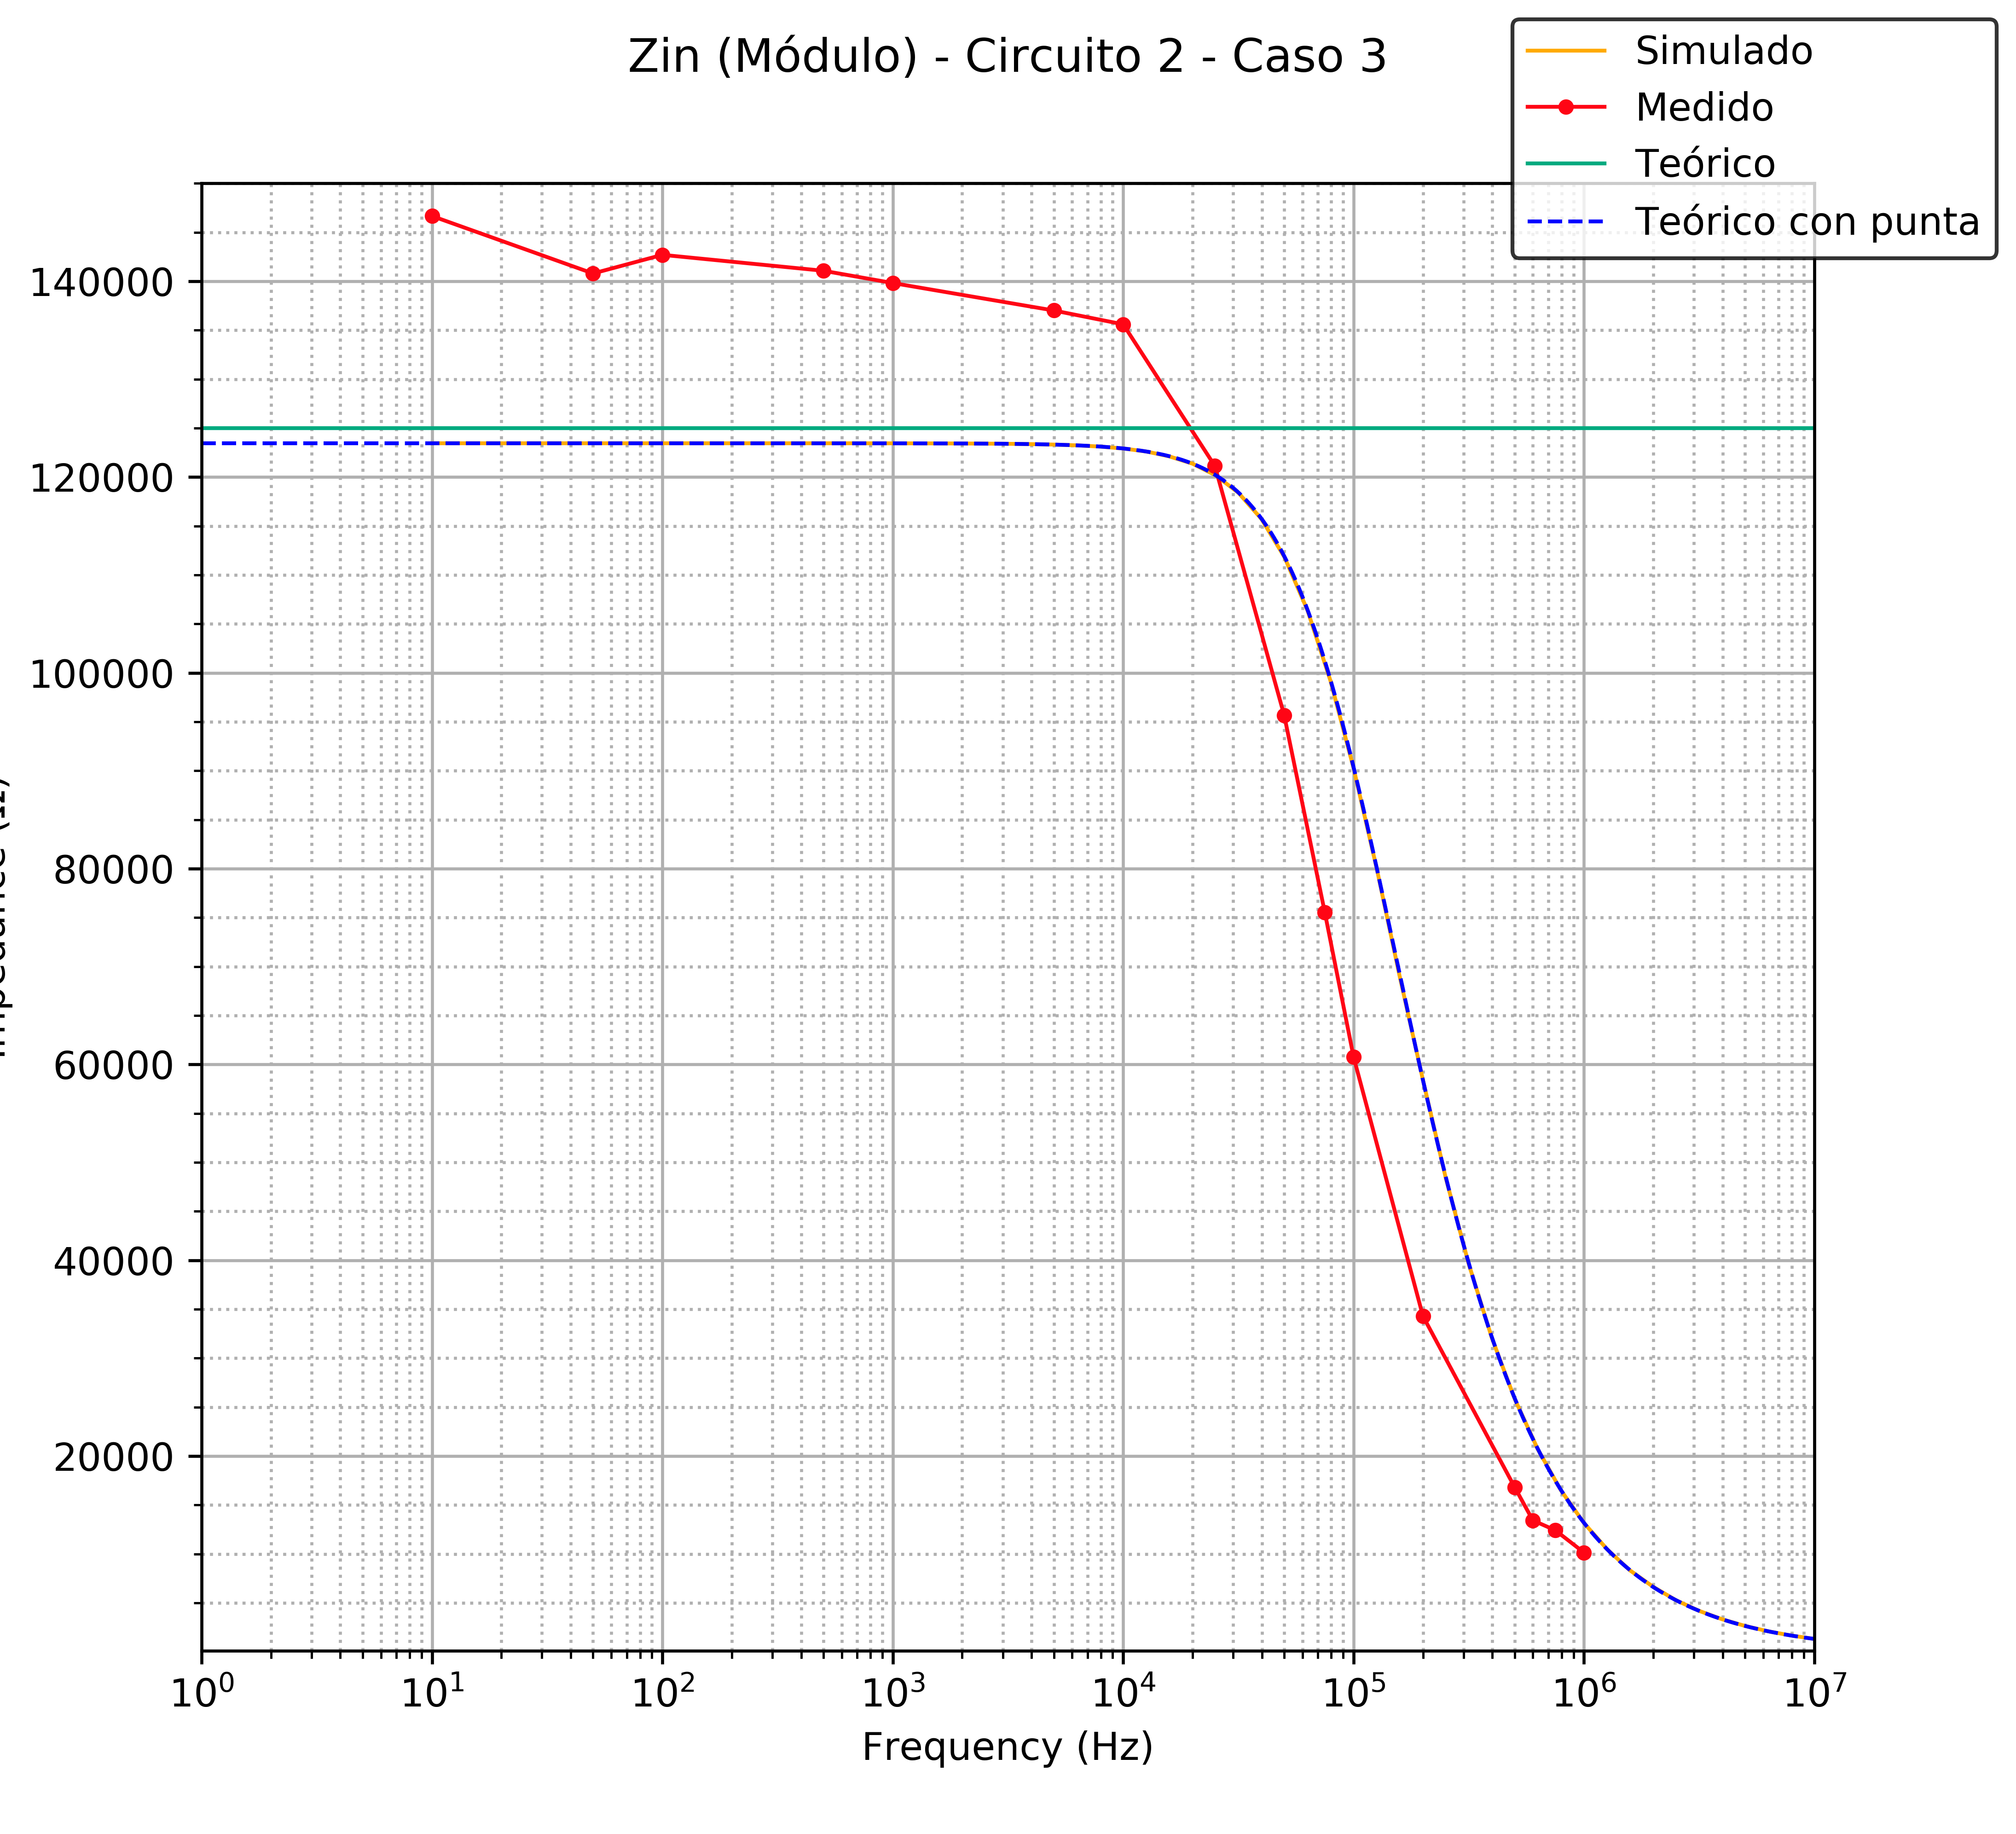
\includegraphics[width=10cm,height=10cm,keepaspectratio]{../EJ1/00GRAFICOS/c2c3/c2c3ZINpunta.png}
%	\caption{Configuración no inversora - Caso 3 - M\'odulo de $Z_{in}$}
%	\label{c2c3zinM}
%\end{figure}

\begin{figure}[H] %!ht
	\centering
	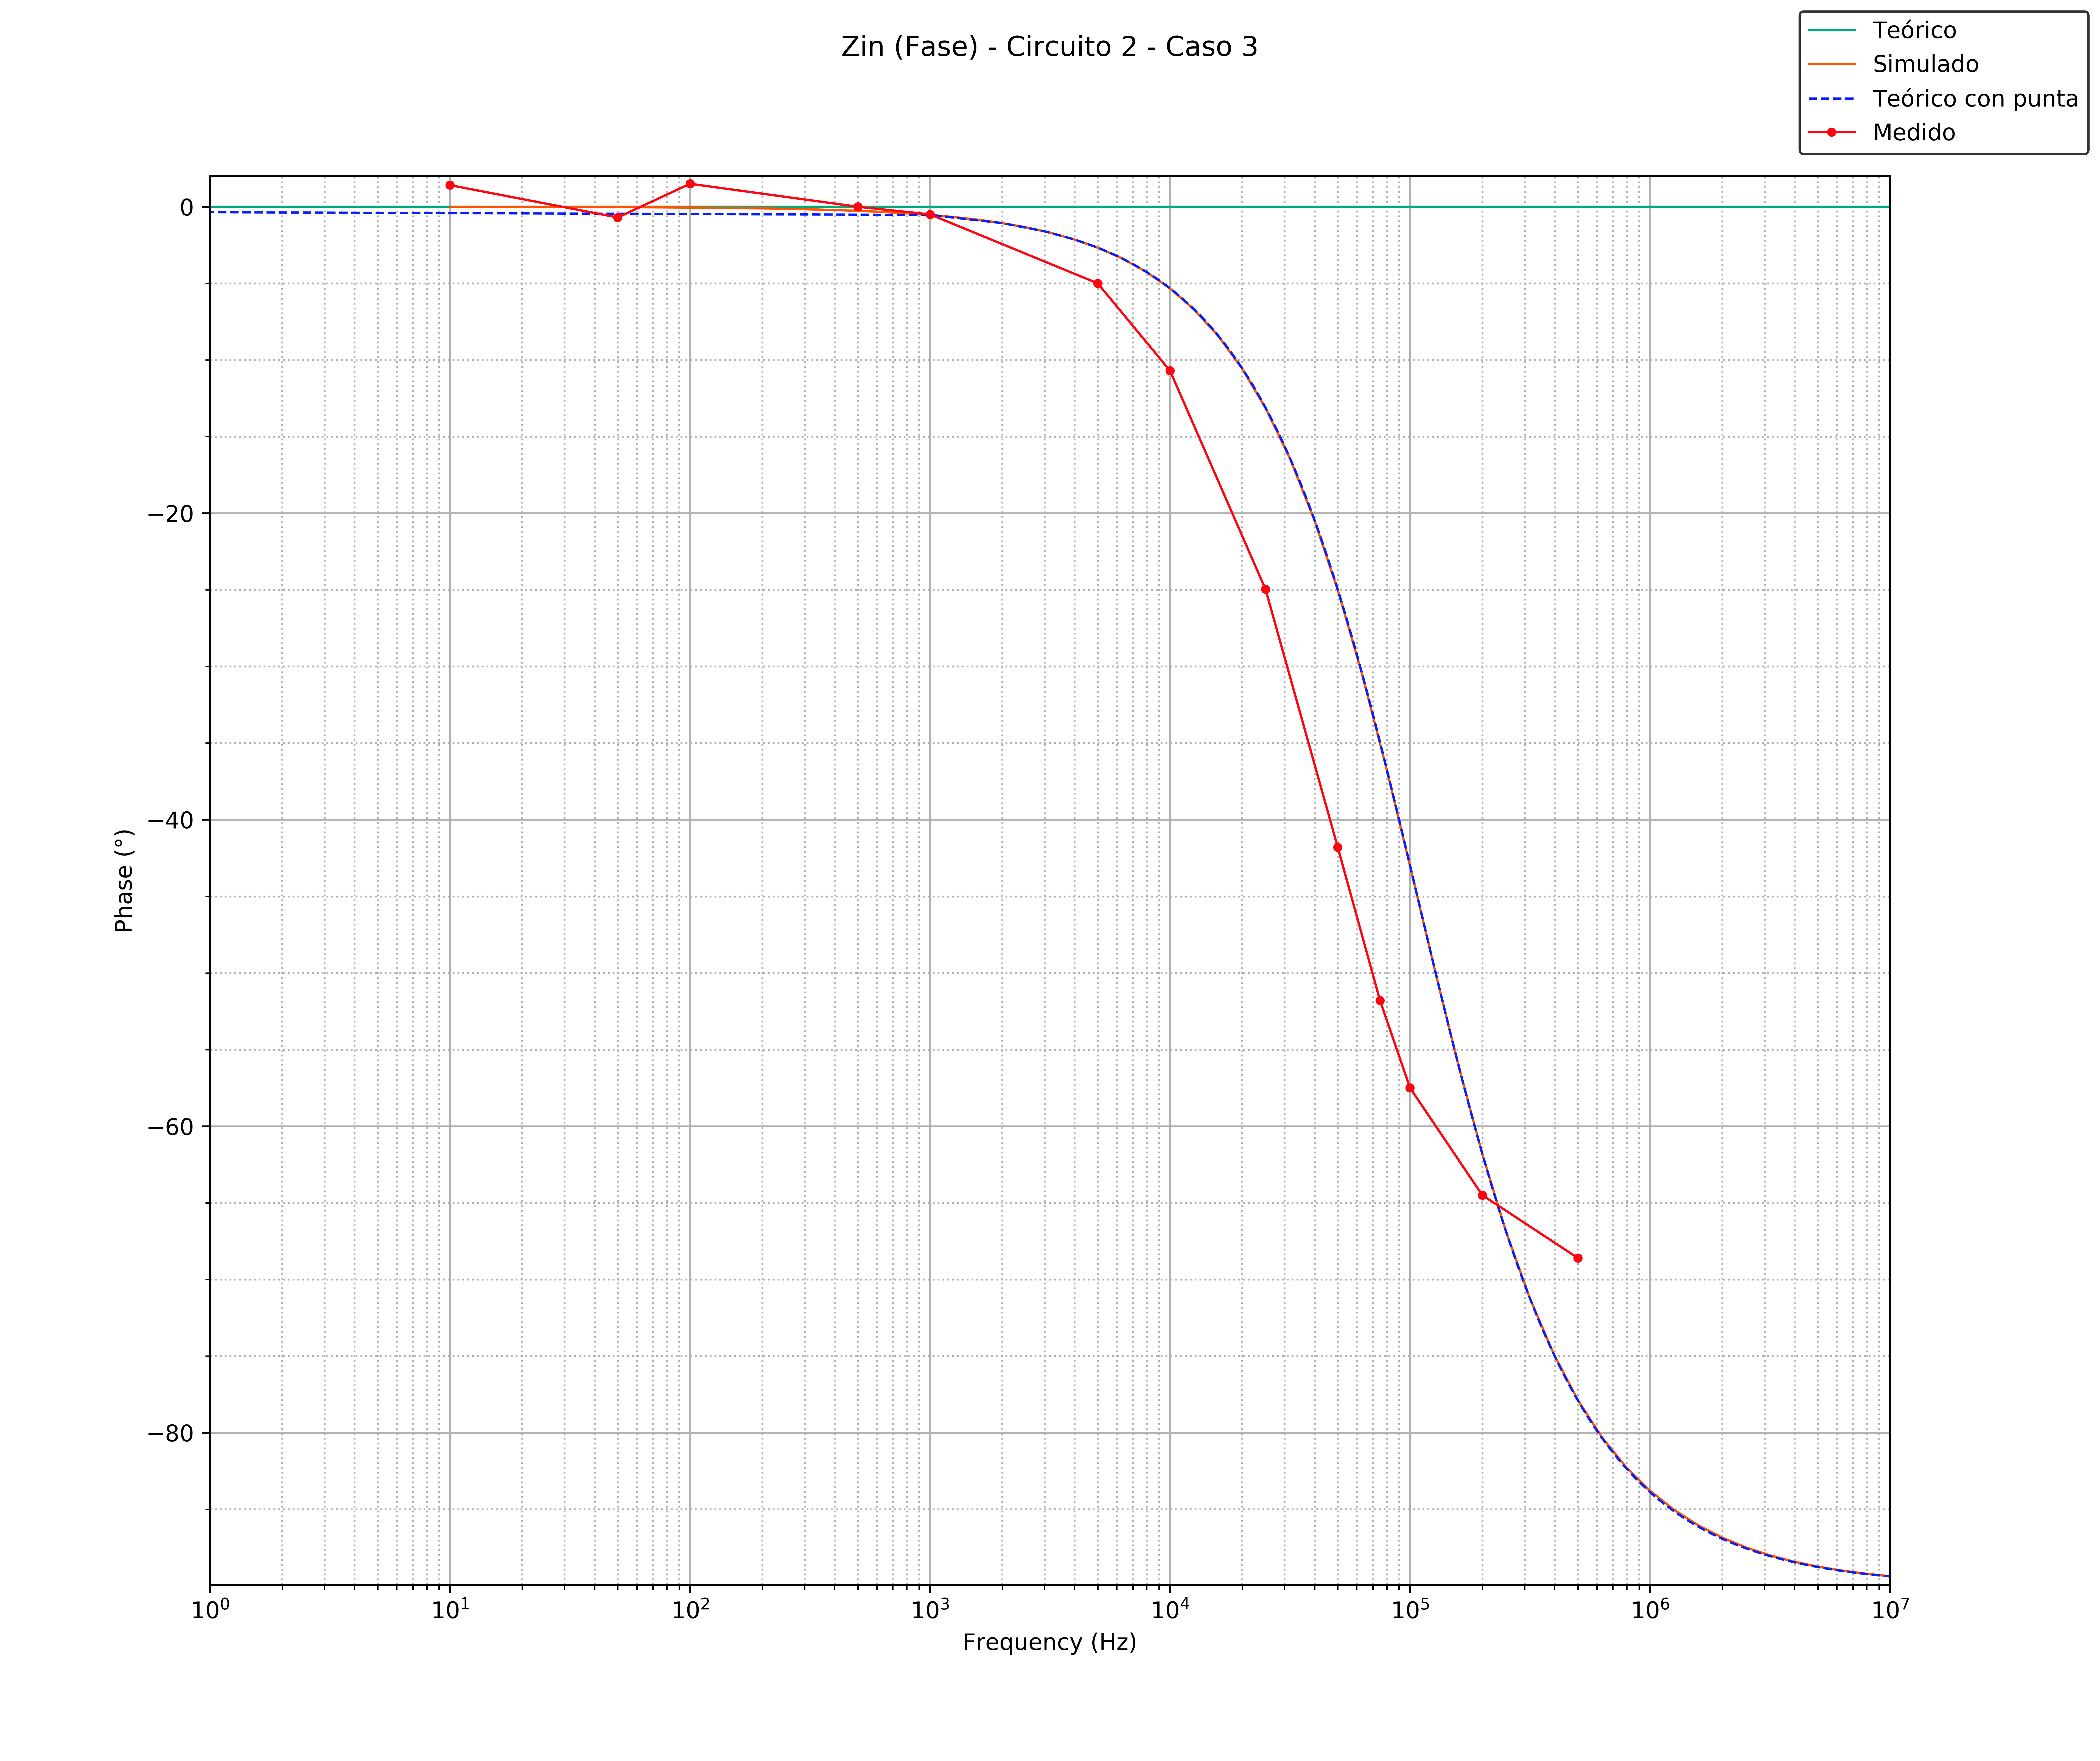
\includegraphics[width=10cm,height=10cm,keepaspectratio]{../EJ1/00GRAFICOS/c2c3/c2c3zinFASE.png}
	\caption{Configuración no inversora - Caso 3 - Fase de $Z_{in}$}
	\label{c2c3zinP}
\end{figure}

Las curvas te\'oricas donde se observa un sobrepico se debe a que no se consideraron las resistencias internas del amplificador operacional en el an\'alisis ya que no estaban en las hojas de datos del mismo. Por lo tanto, habr\'ia que analizar en la expresi\'on te\'orica el $E$ para el cual el pico disminuya y  as\'i se ajustar\'ian aquellas curvas.



